\documentclass[twoside]{book}

% Packages required by doxygen
\usepackage{fixltx2e}
\usepackage{calc}
\usepackage{doxygen}
\usepackage[export]{adjustbox} % also loads graphicx
\usepackage{graphicx}
\usepackage[utf8]{inputenc}
\usepackage{makeidx}
\usepackage{multicol}
\usepackage{multirow}
\PassOptionsToPackage{warn}{textcomp}
\usepackage{textcomp}
\usepackage[nointegrals]{wasysym}
\usepackage[table]{xcolor}

% Font selection
\usepackage[T1]{fontenc}
\usepackage[scaled=.90]{helvet}
\usepackage{courier}
\usepackage{amssymb}
\usepackage{sectsty}
\renewcommand{\familydefault}{\sfdefault}
\allsectionsfont{%
  \fontseries{bc}\selectfont%
  \color{darkgray}%
}
\renewcommand{\DoxyLabelFont}{%
  \fontseries{bc}\selectfont%
  \color{darkgray}%
}
\newcommand{\+}{\discretionary{\mbox{\scriptsize$\hookleftarrow$}}{}{}}

% Page & text layout
\usepackage{geometry}
\geometry{%
  a4paper,%
  top=2.5cm,%
  bottom=2.5cm,%
  left=2.5cm,%
  right=2.5cm%
}
\tolerance=750
\hfuzz=15pt
\hbadness=750
\setlength{\emergencystretch}{15pt}
\setlength{\parindent}{0cm}
\setlength{\parskip}{0.2cm}
\makeatletter
\renewcommand{\paragraph}{%
  \@startsection{paragraph}{4}{0ex}{-1.0ex}{1.0ex}{%
    \normalfont\normalsize\bfseries\SS@parafont%
  }%
}
\renewcommand{\subparagraph}{%
  \@startsection{subparagraph}{5}{0ex}{-1.0ex}{1.0ex}{%
    \normalfont\normalsize\bfseries\SS@subparafont%
  }%
}
\makeatother

% Headers & footers
\usepackage{fancyhdr}
\pagestyle{fancyplain}
\fancyhead[LE]{\fancyplain{}{\bfseries\thepage}}
\fancyhead[CE]{\fancyplain{}{}}
\fancyhead[RE]{\fancyplain{}{\bfseries\leftmark}}
\fancyhead[LO]{\fancyplain{}{\bfseries\rightmark}}
\fancyhead[CO]{\fancyplain{}{}}
\fancyhead[RO]{\fancyplain{}{\bfseries\thepage}}
\fancyfoot[LE]{\fancyplain{}{}}
\fancyfoot[CE]{\fancyplain{}{}}
\fancyfoot[RE]{\fancyplain{}{\bfseries\scriptsize Generated on Mon Jan 19 2015 11\+:19\+:25 for nymeria\+\_\+ardrone by Doxygen }}
\fancyfoot[LO]{\fancyplain{}{\bfseries\scriptsize Generated on Mon Jan 19 2015 11\+:19\+:25 for nymeria\+\_\+ardrone by Doxygen }}
\fancyfoot[CO]{\fancyplain{}{}}
\fancyfoot[RO]{\fancyplain{}{}}
\renewcommand{\footrulewidth}{0.4pt}
\renewcommand{\chaptermark}[1]{%
  \markboth{#1}{}%
}
\renewcommand{\sectionmark}[1]{%
  \markright{\thesection\ #1}%
}

% Indices & bibliography
\usepackage{natbib}
\usepackage[titles]{tocloft}
\setcounter{tocdepth}{3}
\setcounter{secnumdepth}{5}
\makeindex

% Hyperlinks (required, but should be loaded last)
\usepackage{ifpdf}
\ifpdf
  \usepackage[pdftex,pagebackref=true]{hyperref}
\else
  \usepackage[ps2pdf,pagebackref=true]{hyperref}
\fi
\hypersetup{%
  colorlinks=true,%
  linkcolor=blue,%
  citecolor=blue,%
  unicode%
}

% Custom commands
\newcommand{\clearemptydoublepage}{%
  \newpage{\pagestyle{empty}\cleardoublepage}%
}


%===== C O N T E N T S =====

\begin{document}

% Titlepage & ToC
\hypersetup{pageanchor=false,
             bookmarks=true,
             bookmarksnumbered=true,
             pdfencoding=unicode
            }
\pagenumbering{roman}
\begin{titlepage}
\vspace*{7cm}
\begin{center}%
{\Large nymeria\+\_\+ardrone }\\
\vspace*{1cm}
{\large Generated by Doxygen 1.8.9.1}\\
\vspace*{0.5cm}
{\small Mon Jan 19 2015 11:19:25}\\
\end{center}
\end{titlepage}
\clearemptydoublepage
\tableofcontents
\clearemptydoublepage
\pagenumbering{arabic}
\hypersetup{pageanchor=true}

%--- Begin generated contents ---
\chapter{Main Page}
\label{index}\hypertarget{index}{}nymeria\+\_\+ardrone is a \href{http://ros.org/}{\tt R\+O\+S} package for \href{http://ardrone2.parrot.com/}{\tt Parrot A\+R-\/\+Drone} quadrocopter. It acts as a layer and filters drone commands sent from an external controller. It helps the drone determine if movement orders are safe or not depending on the trajectory of an obstacle and, if so, to move accordingly. In practice it contains three main modules. The first, linked to sensors, allows the drone to detect an obstacle. The second gets drone commands and the last makes the link between them. User defines radius of an obstacle and drone is controlled by \hyperlink{class_nymeria}{Nymeria} to slow down and stop in front of it. The driver supports A\+R-\/\+Drone 2.\+0.

\subsection*{Table of Contents}


\begin{DoxyItemize}
\item \href{#requirements}{\tt Requirements}
\item \href{#installation}{\tt Installation}
\item \href{#how-to-run}{\tt How to run it}
\item \href{#how-does-it-work}{\tt How does it work}
\end{DoxyItemize}

\subsection*{Requirements}


\begin{DoxyItemize}
\item {\itshape R\+O\+S}\+: \href{http://wiki.ros.org/ROS/Installation}{\tt Robot Operating System}
\item {\itshape ardrone\+\_\+autonomy}\+: \href{https://github.com/AutonomyLab/ardrone_autonomy}{\tt Driver for Ardrone 1.\+0 \& 2.\+0}
\item {\itshape Sensor}\+: any kind of tool enabling to retrieve range between drone and front obstacles
\end{DoxyItemize}

\subsection*{Installation}

The first step is to install R\+O\+S following the \href{http://wiki.ros.org/ROS/Installation}{\tt (Robot Operating System installation tutorial)}. We have successfully tested two versions \+: hydro and indigo.

Then create a \href{http://wiki.ros.org/ROS/Tutorials/InstallingandConfiguringROSEnvironment#Create_a_ROS_Workspace}{\tt R\+O\+S workspace}.

In order to communicate with the drone you will need to download \href{https://github.com/AutonomyLab/ardrone_autonomy}{\tt ardrone\+\_\+autonomy} which provide the ardrone\+\_\+driver. Follow the instruction in the \href{https://github.com/AutonomyLab/ardrone_autonomy#installation}{\tt installation section}.

Navigate to your catkin\+\_\+workspace sources repository. \begin{quote}
\$ cd $\sim$/catkin\+\_\+ws/src \end{quote}


Download the nymeria\+\_\+ardrone package using the following command in a terminal. \begin{quote}
\$ git clone \href{https://github.com/jdufant/nymeria_ardrone}{\tt https\+://github.\+com/jdufant/nymeria\+\_\+ardrone} \end{quote}


You might prefer to reach \href{https://github.com/jdufant/nymeria_ardrone}{\tt nymeria\+\_\+ardrone webpage} and download and unpack the nymeria\+\_\+ardrone package.

Go back to your root workspace repository. \begin{quote}
\$ cd $\sim$/catkin\+\_\+ws \end{quote}


Use the catkin\+\_\+make command to compile \begin{quote}
\$ catkin\+\_\+make \end{quote}


\subsection*{How to run it}

First switch on Wifi on your computer and connect it to your Ardrone 2.\+0.

You must launch the master node. Navigate to your catkin\+\_\+workspace ({\ttfamily \$ cd $\sim$/catkin\+\_\+ws}) and type the following command \+: \begin{quote}
\$ roscore \end{quote}


Then launch the ardrone\+\_\+autonomy driver\textquotesingle{}s executable node. You can use \+: \begin{quote}
\$ rosrun ardrone\+\_\+autonomy ardrone\+\_\+driver \end{quote}


Or put it in a custom launch file with your desired parameters.

Navigate to $\sim$/catkin\+\_\+ws/src/nymeria\+\_\+ardrone/src/\+Sensor\+Interface.cpp and find the line {\itshape nco.\+input\+Cur\+Front\+Dist(cut\+Value);} Replace the \textquotesingle{}cut\+Value\textquotesingle{} variable by the current distance of the front sensor of your drone. Once done, run the sensor\+\_\+interface node \+: \begin{quote}
\$ rosrun nymeria\+\_\+ardrone nymeria\+\_\+sensor\+\_\+interface \end{quote}


By default the security distance is 100 cm. To change it just call the set\+Security\+Dist(double sec\+Dist) from the class \hyperlink{class_nymeria_check_obstacle}{Nymeria\+Check\+Obstacle}. 
\begin{DoxyCode}
\textcolor{keywordtype}{double} getSecurityDist();
\textcolor{keywordtype}{void} setSecurityDist(\textcolor{keywordtype}{double} secDist);
\end{DoxyCode}


By default the sensor max range is 350 cm. To change it just call the set\+Sensor\+Max\+Range(double range) from the class \hyperlink{class_nymeria_check_obstacle}{Nymeria\+Check\+Obstacle}. 
\begin{DoxyCode}
\textcolor{keywordtype}{double} getSensorMaxRange();
\textcolor{keywordtype}{void} setSensorMaxRange(\textcolor{keywordtype}{double} range);
\end{DoxyCode}


Launch the nymeria\+\_\+command executable node using \+: \begin{quote}
\$ rosrun nymeria\+\_\+ardrone nymeria\+\_\+command \end{quote}


This node is the interface between you as a user who wish to send orders and the drone. Command are sent from keystroke detailled below.
\begin{DoxyItemize}
\item {\itshape E\+N\+T\+E\+R} \+: L\+A\+N\+D / T\+A\+K\+E O\+F\+F
\item {\itshape Z} \+: move forward
\item {\itshape S} \+: move backward
\item {\itshape Q} \+: rotate left
\item {\itshape D} \+: rotate right
\item {\itshape U\+P} \+: move up
\item {\itshape D\+O\+W\+N} \+: move down
\item {\itshape i} \+: move down
\item {\itshape k} \+: move down
\item {\itshape o} \+: move down
\item {\itshape l} \+: move down
\item {\itshape p} \+: move down
\item {\itshape m} \+: move down
\item {\itshape S\+P\+A\+C\+E} \+: stop
\end{DoxyItemize}

The last step consists to run the launch the Controller node \begin{quote}
\$ rosrun nymeria\+\_\+ardrone controller \end{quote}


You are ready to go. Just stroke the appropriate key from the nymeria\+\_\+command interface. Your drone will naturally keep the inputed security distance between any front obstacle and itself.

\subsection*{How does it work}
\chapter{Hierarchical Index}
\section{\-Class \-Hierarchy}
\-This inheritance list is sorted roughly, but not completely, alphabetically\-:\begin{DoxyCompactList}
\item \contentsline{section}{\-Controller}{\pageref{classController}}{}
\item \contentsline{section}{\-Nymeria}{\pageref{classNymeria}}{}
\item \contentsline{section}{\-Nymeria\-Check\-Obstacle}{\pageref{classNymeriaCheckObstacle}}{}
\item \contentsline{section}{\-Nymeria\-Constants}{\pageref{classNymeriaConstants}}{}
\item \contentsline{section}{\-Nymeria\-Exceptions}{\pageref{classNymeriaExceptions}}{}
\begin{DoxyCompactList}
\item \contentsline{section}{\-Nymeria\-Invalid\-Security\-Distance}{\pageref{classNymeriaInvalidSecurityDistance}}{}
\item \contentsline{section}{\-Nymeria\-Param\-Exc}{\pageref{classNymeriaParamExc}}{}
\end{DoxyCompactList}
\item \contentsline{section}{\-Nymeria\-Mutex}{\pageref{classNymeriaMutex}}{}
\begin{DoxyCompactList}
\item \contentsline{section}{\-Nymeria\-Mutex\-Command}{\pageref{classNymeriaMutexCommand}}{}
\item \contentsline{section}{\-Nymeria\-Mutex\-Obstacle}{\pageref{classNymeriaMutexObstacle}}{}
\item \contentsline{section}{\-Nymeria\-Mutex\-Security\-Distance}{\pageref{classNymeriaMutexSecurityDistance}}{}
\end{DoxyCompactList}
\item \contentsline{section}{\-Sensor\-Interface}{\pageref{classSensorInterface}}{}
\item \contentsline{section}{\-Teleop\-Keyboard}{\pageref{classTeleopKeyboard}}{}
\item \contentsline{section}{\-U\-D\-P\-Client}{\pageref{classUDPClient}}{}
\item \contentsline{section}{\-U\-D\-P\-Server}{\pageref{classUDPServer}}{}
\end{DoxyCompactList}

\chapter{Class Index}
\section{Class List}
Here are the classes, structs, unions and interfaces with brief descriptions\+:\begin{DoxyCompactList}
\item\contentsline{section}{\hyperlink{class_nymeria}{Nymeria} \\*Definitions of the class \hyperlink{class_nymeria}{Nymeria}, that declares all functionalities in order to allow for drone navigation with obstacle detection and avoidance }{\pageref{class_nymeria}}{}
\item\contentsline{section}{\hyperlink{class_nymeria_check_obstacle}{Nymeria\+Check\+Obstacle} }{\pageref{class_nymeria_check_obstacle}}{}
\item\contentsline{section}{\hyperlink{class_nymeria_constants}{Nymeria\+Constants} \\*Declaration of the class \hyperlink{class_nymeria_constants}{Nymeria\+Constants}, that defines all constants necessary to define both commands and states of the drone and obstacles }{\pageref{class_nymeria_constants}}{}
\item\contentsline{section}{\hyperlink{class_nymeria_exceptions}{Nymeria\+Exceptions} \\*Declaration of the class \hyperlink{class_nymeria_exceptions}{Nymeria\+Exceptions}, that declares the base class for all exceptions particular to \hyperlink{class_nymeria}{Nymeria} }{\pageref{class_nymeria_exceptions}}{}
\item\contentsline{section}{\hyperlink{class_nymeria_invalid_security_distance}{Nymeria\+Invalid\+Security\+Distance} \\*Declaration of the class \hyperlink{class_nymeria_param_exc}{Nymeria\+Param\+Exc}, that declares the exception thrown when the R\+O\+S parameter requested does not exist or was misspelled }{\pageref{class_nymeria_invalid_security_distance}}{}
\item\contentsline{section}{\hyperlink{class_nymeria_mutex}{Nymeria\+Mutex} }{\pageref{class_nymeria_mutex}}{}
\item\contentsline{section}{\hyperlink{class_nymeria_mutex_command}{Nymeria\+Mutex\+Command} }{\pageref{class_nymeria_mutex_command}}{}
\item\contentsline{section}{\hyperlink{class_nymeria_mutex_obstacle}{Nymeria\+Mutex\+Obstacle} }{\pageref{class_nymeria_mutex_obstacle}}{}
\item\contentsline{section}{\hyperlink{class_nymeria_mutex_security_distance}{Nymeria\+Mutex\+Security\+Distance} }{\pageref{class_nymeria_mutex_security_distance}}{}
\item\contentsline{section}{\hyperlink{class_nymeria_param_exc}{Nymeria\+Param\+Exc} \\*Declaration of the class \hyperlink{class_nymeria_param_exc}{Nymeria\+Param\+Exc}, that declares the exception thrown when the R\+O\+S parameter requested does not exist or was misspelled }{\pageref{class_nymeria_param_exc}}{}
\end{DoxyCompactList}

\chapter{File Index}
\section{File List}
Here is a list of all files with brief descriptions\+:\begin{DoxyCompactList}
\item\contentsline{section}{include/nymeria\+\_\+ardrone/\hyperlink{_nymeria_8h}{Nymeria.\+h} }{\pageref{_nymeria_8h}}{}
\item\contentsline{section}{include/nymeria\+\_\+ardrone/\hyperlink{_nymeria_check_obstacle_8h}{Nymeria\+Check\+Obstacle.\+h} }{\pageref{_nymeria_check_obstacle_8h}}{}
\item\contentsline{section}{include/nymeria\+\_\+ardrone/\hyperlink{_nymeria_constants_8h}{Nymeria\+Constants.\+h} }{\pageref{_nymeria_constants_8h}}{}
\item\contentsline{section}{include/nymeria\+\_\+ardrone/\hyperlink{_nymeria_exceptions_8h}{Nymeria\+Exceptions.\+h} }{\pageref{_nymeria_exceptions_8h}}{}
\item\contentsline{section}{include/nymeria\+\_\+ardrone/\hyperlink{_nymeria_invalid_security_distance_8h}{Nymeria\+Invalid\+Security\+Distance.\+h} }{\pageref{_nymeria_invalid_security_distance_8h}}{}
\item\contentsline{section}{include/nymeria\+\_\+ardrone/\hyperlink{_nymeria_mutex_8h}{Nymeria\+Mutex.\+h} }{\pageref{_nymeria_mutex_8h}}{}
\item\contentsline{section}{include/nymeria\+\_\+ardrone/\hyperlink{_nymeria_mutex_command_8h}{Nymeria\+Mutex\+Command.\+h} }{\pageref{_nymeria_mutex_command_8h}}{}
\item\contentsline{section}{include/nymeria\+\_\+ardrone/\hyperlink{_nymeria_mutex_obstacle_8h}{Nymeria\+Mutex\+Obstacle.\+h} }{\pageref{_nymeria_mutex_obstacle_8h}}{}
\item\contentsline{section}{include/nymeria\+\_\+ardrone/\hyperlink{_nymeria_mutex_security_distance_8h}{Nymeria\+Mutex\+Security\+Distance.\+h} }{\pageref{_nymeria_mutex_security_distance_8h}}{}
\item\contentsline{section}{include/nymeria\+\_\+ardrone/\hyperlink{_nymeria_param_exc_8h}{Nymeria\+Param\+Exc.\+h} }{\pageref{_nymeria_param_exc_8h}}{}
\item\contentsline{section}{src/\hyperlink{_nymeria_8cpp}{Nymeria.\+cpp} }{\pageref{_nymeria_8cpp}}{}
\item\contentsline{section}{src/\hyperlink{_nymeria_check_obstacle_8cpp}{Nymeria\+Check\+Obstacle.\+cpp} }{\pageref{_nymeria_check_obstacle_8cpp}}{}
\item\contentsline{section}{src/\hyperlink{_nymeria_constants_8cpp}{Nymeria\+Constants.\+cpp} }{\pageref{_nymeria_constants_8cpp}}{}
\item\contentsline{section}{src/\hyperlink{_nymeria_mutex_8cpp}{Nymeria\+Mutex.\+cpp} }{\pageref{_nymeria_mutex_8cpp}}{}
\item\contentsline{section}{src/\hyperlink{_nymeria_mutex_command_8cpp}{Nymeria\+Mutex\+Command.\+cpp} }{\pageref{_nymeria_mutex_command_8cpp}}{}
\item\contentsline{section}{src/\hyperlink{_nymeria_mutex_obstacle_8cpp}{Nymeria\+Mutex\+Obstacle.\+cpp} }{\pageref{_nymeria_mutex_obstacle_8cpp}}{}
\item\contentsline{section}{src/\hyperlink{_nymeria_mutex_security_distance_8cpp}{Nymeria\+Mutex\+Security\+Distance.\+cpp} }{\pageref{_nymeria_mutex_security_distance_8cpp}}{}
\item\contentsline{section}{src/exception/\hyperlink{_nymeria_exceptions_8cpp}{Nymeria\+Exceptions.\+cpp} }{\pageref{_nymeria_exceptions_8cpp}}{}
\item\contentsline{section}{src/exception/\hyperlink{_nymeria_invalid_security_distance_8cpp}{Nymeria\+Invalid\+Security\+Distance.\+cpp} }{\pageref{_nymeria_invalid_security_distance_8cpp}}{}
\item\contentsline{section}{src/exception/\hyperlink{_nymeria_param_exc_8cpp}{Nymeria\+Param\+Exc.\+cpp} }{\pageref{_nymeria_param_exc_8cpp}}{}
\end{DoxyCompactList}

\chapter{Class Documentation}
\hypertarget{class_nymeria}{}\section{Nymeria Class Reference}
\label{class_nymeria}\index{Nymeria@{Nymeria}}


Definitions of the class \hyperlink{class_nymeria}{Nymeria}, that declares all functionalities in order to allow for drone navigation with obstacle detection and avoidance.  




{\ttfamily \#include $<$Nymeria.\+h$>$}

\subsection*{Public Member Functions}
\begin{DoxyCompactItemize}
\item 
\hyperlink{class_nymeria_acee38ea6f62c9b81a6ec1a2c253456b9}{Nymeria} ()
\begin{DoxyCompactList}\small\item\em Default empty constructor. \end{DoxyCompactList}\item 
\hyperlink{class_nymeria_adaf1ee7808196815ff68489ddeb9b16d}{Nymeria} (ros\+::\+Node\+Handle $\ast$n)
\begin{DoxyCompactList}\small\item\em Constructor in order to create a meaningful object of the type \hyperlink{class_nymeria}{Nymeria}. \end{DoxyCompactList}\item 
void \hyperlink{class_nymeria_a3b35e3472b5335e3cb167fd9f7d28e57}{move\+Forward} ()
\begin{DoxyCompactList}\small\item\em Command in order to move drone forward. \end{DoxyCompactList}\item 
void \hyperlink{class_nymeria_a7781b8726f7a471265f86cd922440b12}{move\+Backward} ()
\begin{DoxyCompactList}\small\item\em Command in order to move drone backward. \end{DoxyCompactList}\item 
void \hyperlink{class_nymeria_a95e1a46cb702df4244a3058de3c19812}{move\+Left} ()
\begin{DoxyCompactList}\small\item\em Command in order to make drone rotate to the left. \end{DoxyCompactList}\item 
void \hyperlink{class_nymeria_a0cf0b3b960e66da1b3761d9df00bf08c}{move\+Right} ()
\begin{DoxyCompactList}\small\item\em Command in order to make drone rotate to the right. \end{DoxyCompactList}\item 
void \hyperlink{class_nymeria_a33ad22560168d804fb4556bf22f37890}{move\+Up} ()
\begin{DoxyCompactList}\small\item\em Command in order to move drone upward, i.\+e. \end{DoxyCompactList}\item 
void \hyperlink{class_nymeria_af317acf40210155d86a451d8498486bb}{move\+Down} ()
\begin{DoxyCompactList}\small\item\em Command in order to move drone downward, i.\+e. \end{DoxyCompactList}\item 
void \hyperlink{class_nymeria_ac5ffdf4e6182fddfc5c082bc3e9c2cff}{turn\+Left} ()
\begin{DoxyCompactList}\small\item\em Command in order to move drone to the left. \end{DoxyCompactList}\item 
void \hyperlink{class_nymeria_a73bc4685c0de47b7a64c168218294765}{turn\+Right} ()
\begin{DoxyCompactList}\small\item\em Command in order to move drone to the right. \end{DoxyCompactList}\item 
void \hyperlink{class_nymeria_ac89e119ce6553bc25a104455159e7dcc}{stop} ()
\begin{DoxyCompactList}\small\item\em Command in order to stop the drone\textquotesingle{}s movement, i.\+e. \end{DoxyCompactList}\item 
void \hyperlink{class_nymeria_ada86813f80111e1e8cec9cbd0e0d3edd}{take\+Off} ()
\begin{DoxyCompactList}\small\item\em Command in order to make the drone take off. \end{DoxyCompactList}\item 
void \hyperlink{class_nymeria_ac552d48476ba1999ce13461bed238bfb}{land} ()
\begin{DoxyCompactList}\small\item\em Command in order to make the drone land, i.\+e. \end{DoxyCompactList}\item 
void \hyperlink{class_nymeria_a871d92e2206ca9ceb768b1bc35b83e8d}{emergency\+Stop} ()
\begin{DoxyCompactList}\small\item\em Command in order to make drone stop and immediately land. \end{DoxyCompactList}\item 
void \hyperlink{class_nymeria_af0bf1c66411d398b7ffed2ce05b6d521}{increase\+Max\+Linear\+Speed} ()
\begin{DoxyCompactList}\small\item\em Command in order to increase the maximum linear speed by 10\%. \end{DoxyCompactList}\item 
void \hyperlink{class_nymeria_a3d7885e178ab495a79f4d7c6820b703a}{decrease\+Max\+Linear\+Speed} ()
\begin{DoxyCompactList}\small\item\em Command in order to decrease the maximum linear speed by 10\%. \end{DoxyCompactList}\item 
void \hyperlink{class_nymeria_abb97d909934b058ee3bf9d3e9090ad95}{increase\+Max\+Angular\+Speed} ()
\begin{DoxyCompactList}\small\item\em Command in order to increase the maximum angular speed by 10\%. \end{DoxyCompactList}\item 
void \hyperlink{class_nymeria_a32c636fb95fcf32793f7632c4675b57c}{decrease\+Max\+Angular\+Speed} ()
\begin{DoxyCompactList}\small\item\em Command in order to decrease the maximum angular speed by 10\%. \end{DoxyCompactList}\item 
void \hyperlink{class_nymeria_a9fdb89e4e84a7ad566b7d0e1e06c17a0}{increase\+Linear\+Speed} ()
\begin{DoxyCompactList}\small\item\em Command in order to increase the linear speed by 10\%. \end{DoxyCompactList}\item 
void \hyperlink{class_nymeria_a08983812723252986961fb810eb875f4}{decrease\+Linear\+Speed} ()
\begin{DoxyCompactList}\small\item\em Command in order to decrease the linear speed by 10\%. \end{DoxyCompactList}\item 
void \hyperlink{class_nymeria_ad96f2f3ef25a0d466e2866ee020d0d57}{increase\+Angular\+Speed} ()
\begin{DoxyCompactList}\small\item\em Command in order to increase the angular speed by 10\%. \end{DoxyCompactList}\item 
void \hyperlink{class_nymeria_a354a426d9626623eb60f59bea93cf888}{decrease\+Angular\+Speed} ()
\begin{DoxyCompactList}\small\item\em Command in order to decrease the angular speed by 10\%. \end{DoxyCompactList}\item 
double \hyperlink{class_nymeria_a39846f73d57a98ab24a80a80be38ddef}{get\+Security\+Dist} ()
\begin{DoxyCompactList}\small\item\em Getter function for security distance, in order to permit the user to retain its current value. \end{DoxyCompactList}\item 
void \hyperlink{class_nymeria_af145b44f01dc82ba70f3b09bc459364d}{set\+Security\+Dist} (double sec\+Dist)
\begin{DoxyCompactList}\small\item\em Setter function for security distance, in order to permit the user to change its value. \end{DoxyCompactList}\item 
double \hyperlink{class_nymeria_adce898b1df4cdfe04a3dd6fca7745f36}{get\+Max\+Linear\+Speed} ()
\begin{DoxyCompactList}\small\item\em Getter function for maximum linear speed, in order to permit the user to retain its current value. \end{DoxyCompactList}\item 
void \hyperlink{class_nymeria_a97fb26da752c0ac03b4f0874f9513e01}{set\+Max\+Linear\+Speed} (double speed)
\begin{DoxyCompactList}\small\item\em Setter function for maximum linear speed, in order to permit the user to change its value. \end{DoxyCompactList}\item 
double \hyperlink{class_nymeria_a791c7e89a7044302557f7f1dbd6f6f84}{get\+Linear\+Speed} ()
\begin{DoxyCompactList}\small\item\em Getter function for current linear speed. \end{DoxyCompactList}\item 
void \hyperlink{class_nymeria_a6217513fd20574947ec6ca0405668c1a}{set\+Linear\+Speed} (double speed)
\begin{DoxyCompactList}\small\item\em Setter function for current linear speed, in order to permit the user to change its value. \end{DoxyCompactList}\item 
double \hyperlink{class_nymeria_abee78301bcaf62d61f2777aa2c5b9449}{get\+Max\+Angular\+Speed} ()
\begin{DoxyCompactList}\small\item\em Getter function for maximum angular speed, in order to permit the user to retain its current value. \end{DoxyCompactList}\item 
void \hyperlink{class_nymeria_a8f4694ca2039c6893706566b8b368833}{set\+Max\+Angular\+Speed} (double speed)
\begin{DoxyCompactList}\small\item\em Setter function for maximum angular speed, in order to permit the user to change its value. \end{DoxyCompactList}\item 
double \hyperlink{class_nymeria_a5020233162c927226ff48dc211dbb225}{get\+Angular\+Speed} ()
\begin{DoxyCompactList}\small\item\em Getter function for angular speed, in order to permit the user to retain its current value. \end{DoxyCompactList}\end{DoxyCompactItemize}
\subsection*{Friends}
\begin{DoxyCompactItemize}
\item 
class \hyperlink{class_nymeria_ac3456fd331a58b288082abca310c7a99}{Controller}
\end{DoxyCompactItemize}


\subsection{Detailed Description}
Definitions of the class \hyperlink{class_nymeria}{Nymeria}, that declares all functionalities in order to allow for drone navigation with obstacle detection and avoidance. 

\begin{DoxyAuthor}{Author}
Team-\/\+Nymeria 
\end{DoxyAuthor}
\begin{DoxyVersion}{Version}
0.\+2 
\end{DoxyVersion}
\begin{DoxyDate}{Date}
18th of January 2015 
\end{DoxyDate}


\subsection{Constructor \& Destructor Documentation}
\hypertarget{class_nymeria_acee38ea6f62c9b81a6ec1a2c253456b9}{}\index{Nymeria@{Nymeria}!Nymeria@{Nymeria}}
\index{Nymeria@{Nymeria}!Nymeria@{Nymeria}}
\subsubsection[{Nymeria}]{\setlength{\rightskip}{0pt plus 5cm}Nymeria\+::\+Nymeria (
\begin{DoxyParamCaption}
{}
\end{DoxyParamCaption}
)}\label{class_nymeria_acee38ea6f62c9b81a6ec1a2c253456b9}


Default empty constructor. 

\hypertarget{class_nymeria_adaf1ee7808196815ff68489ddeb9b16d}{}\index{Nymeria@{Nymeria}!Nymeria@{Nymeria}}
\index{Nymeria@{Nymeria}!Nymeria@{Nymeria}}
\subsubsection[{Nymeria}]{\setlength{\rightskip}{0pt plus 5cm}Nymeria\+::\+Nymeria (
\begin{DoxyParamCaption}
\item[{ros\+::\+Node\+Handle $\ast$}]{n}
\end{DoxyParamCaption}
)}\label{class_nymeria_adaf1ee7808196815ff68489ddeb9b16d}


Constructor in order to create a meaningful object of the type \hyperlink{class_nymeria}{Nymeria}. 

Meaningful in terms of functionality\+: It provides all navigation commands for the drone whilst ensuring obstacle protection and avoidance. 
\begin{DoxyParams}{Parameters}
{\em n} & Node\+Handle permitting to relate R\+O\+S-\/node. \\
\hline
\end{DoxyParams}


\subsection{Member Function Documentation}
\hypertarget{class_nymeria_a354a426d9626623eb60f59bea93cf888}{}\index{Nymeria@{Nymeria}!decrease\+Angular\+Speed@{decrease\+Angular\+Speed}}
\index{decrease\+Angular\+Speed@{decrease\+Angular\+Speed}!Nymeria@{Nymeria}}
\subsubsection[{decrease\+Angular\+Speed}]{\setlength{\rightskip}{0pt plus 5cm}void Nymeria\+::decrease\+Angular\+Speed (
\begin{DoxyParamCaption}
{}
\end{DoxyParamCaption}
)}\label{class_nymeria_a354a426d9626623eb60f59bea93cf888}


Command in order to decrease the angular speed by 10\%. 

\hypertarget{class_nymeria_a08983812723252986961fb810eb875f4}{}\index{Nymeria@{Nymeria}!decrease\+Linear\+Speed@{decrease\+Linear\+Speed}}
\index{decrease\+Linear\+Speed@{decrease\+Linear\+Speed}!Nymeria@{Nymeria}}
\subsubsection[{decrease\+Linear\+Speed}]{\setlength{\rightskip}{0pt plus 5cm}void Nymeria\+::decrease\+Linear\+Speed (
\begin{DoxyParamCaption}
{}
\end{DoxyParamCaption}
)}\label{class_nymeria_a08983812723252986961fb810eb875f4}


Command in order to decrease the linear speed by 10\%. 

\hypertarget{class_nymeria_a32c636fb95fcf32793f7632c4675b57c}{}\index{Nymeria@{Nymeria}!decrease\+Max\+Angular\+Speed@{decrease\+Max\+Angular\+Speed}}
\index{decrease\+Max\+Angular\+Speed@{decrease\+Max\+Angular\+Speed}!Nymeria@{Nymeria}}
\subsubsection[{decrease\+Max\+Angular\+Speed}]{\setlength{\rightskip}{0pt plus 5cm}void Nymeria\+::decrease\+Max\+Angular\+Speed (
\begin{DoxyParamCaption}
{}
\end{DoxyParamCaption}
)}\label{class_nymeria_a32c636fb95fcf32793f7632c4675b57c}


Command in order to decrease the maximum angular speed by 10\%. 

\hypertarget{class_nymeria_a3d7885e178ab495a79f4d7c6820b703a}{}\index{Nymeria@{Nymeria}!decrease\+Max\+Linear\+Speed@{decrease\+Max\+Linear\+Speed}}
\index{decrease\+Max\+Linear\+Speed@{decrease\+Max\+Linear\+Speed}!Nymeria@{Nymeria}}
\subsubsection[{decrease\+Max\+Linear\+Speed}]{\setlength{\rightskip}{0pt plus 5cm}void Nymeria\+::decrease\+Max\+Linear\+Speed (
\begin{DoxyParamCaption}
{}
\end{DoxyParamCaption}
)}\label{class_nymeria_a3d7885e178ab495a79f4d7c6820b703a}


Command in order to decrease the maximum linear speed by 10\%. 

\hypertarget{class_nymeria_a871d92e2206ca9ceb768b1bc35b83e8d}{}\index{Nymeria@{Nymeria}!emergency\+Stop@{emergency\+Stop}}
\index{emergency\+Stop@{emergency\+Stop}!Nymeria@{Nymeria}}
\subsubsection[{emergency\+Stop}]{\setlength{\rightskip}{0pt plus 5cm}void Nymeria\+::emergency\+Stop (
\begin{DoxyParamCaption}
{}
\end{DoxyParamCaption}
)}\label{class_nymeria_a871d92e2206ca9ceb768b1bc35b83e8d}


Command in order to make drone stop and immediately land. 

\hypertarget{class_nymeria_a5020233162c927226ff48dc211dbb225}{}\index{Nymeria@{Nymeria}!get\+Angular\+Speed@{get\+Angular\+Speed}}
\index{get\+Angular\+Speed@{get\+Angular\+Speed}!Nymeria@{Nymeria}}
\subsubsection[{get\+Angular\+Speed}]{\setlength{\rightskip}{0pt plus 5cm}double Nymeria\+::get\+Angular\+Speed (
\begin{DoxyParamCaption}
{}
\end{DoxyParamCaption}
)}\label{class_nymeria_a5020233162c927226ff48dc211dbb225}


Getter function for angular speed, in order to permit the user to retain its current value. 

\begin{DoxyReturn}{Returns}
angular speed 
\end{DoxyReturn}
\hypertarget{class_nymeria_a791c7e89a7044302557f7f1dbd6f6f84}{}\index{Nymeria@{Nymeria}!get\+Linear\+Speed@{get\+Linear\+Speed}}
\index{get\+Linear\+Speed@{get\+Linear\+Speed}!Nymeria@{Nymeria}}
\subsubsection[{get\+Linear\+Speed}]{\setlength{\rightskip}{0pt plus 5cm}double Nymeria\+::get\+Linear\+Speed (
\begin{DoxyParamCaption}
{}
\end{DoxyParamCaption}
)}\label{class_nymeria_a791c7e89a7044302557f7f1dbd6f6f84}


Getter function for current linear speed. 

\begin{DoxyReturn}{Returns}
current linear speed. 
\end{DoxyReturn}
\hypertarget{class_nymeria_abee78301bcaf62d61f2777aa2c5b9449}{}\index{Nymeria@{Nymeria}!get\+Max\+Angular\+Speed@{get\+Max\+Angular\+Speed}}
\index{get\+Max\+Angular\+Speed@{get\+Max\+Angular\+Speed}!Nymeria@{Nymeria}}
\subsubsection[{get\+Max\+Angular\+Speed}]{\setlength{\rightskip}{0pt plus 5cm}double Nymeria\+::get\+Max\+Angular\+Speed (
\begin{DoxyParamCaption}
{}
\end{DoxyParamCaption}
)}\label{class_nymeria_abee78301bcaf62d61f2777aa2c5b9449}


Getter function for maximum angular speed, in order to permit the user to retain its current value. 

\begin{DoxyReturn}{Returns}
maximum angular speed 
\end{DoxyReturn}
\hypertarget{class_nymeria_adce898b1df4cdfe04a3dd6fca7745f36}{}\index{Nymeria@{Nymeria}!get\+Max\+Linear\+Speed@{get\+Max\+Linear\+Speed}}
\index{get\+Max\+Linear\+Speed@{get\+Max\+Linear\+Speed}!Nymeria@{Nymeria}}
\subsubsection[{get\+Max\+Linear\+Speed}]{\setlength{\rightskip}{0pt plus 5cm}double Nymeria\+::get\+Max\+Linear\+Speed (
\begin{DoxyParamCaption}
{}
\end{DoxyParamCaption}
)}\label{class_nymeria_adce898b1df4cdfe04a3dd6fca7745f36}


Getter function for maximum linear speed, in order to permit the user to retain its current value. 

\begin{DoxyReturn}{Returns}
maximum linear speed. 
\end{DoxyReturn}
\hypertarget{class_nymeria_a39846f73d57a98ab24a80a80be38ddef}{}\index{Nymeria@{Nymeria}!get\+Security\+Dist@{get\+Security\+Dist}}
\index{get\+Security\+Dist@{get\+Security\+Dist}!Nymeria@{Nymeria}}
\subsubsection[{get\+Security\+Dist}]{\setlength{\rightskip}{0pt plus 5cm}double Nymeria\+::get\+Security\+Dist (
\begin{DoxyParamCaption}
{}
\end{DoxyParamCaption}
)}\label{class_nymeria_a39846f73d57a98ab24a80a80be38ddef}


Getter function for security distance, in order to permit the user to retain its current value. 

\begin{DoxyReturn}{Returns}
security distance. 
\end{DoxyReturn}
\hypertarget{class_nymeria_ad96f2f3ef25a0d466e2866ee020d0d57}{}\index{Nymeria@{Nymeria}!increase\+Angular\+Speed@{increase\+Angular\+Speed}}
\index{increase\+Angular\+Speed@{increase\+Angular\+Speed}!Nymeria@{Nymeria}}
\subsubsection[{increase\+Angular\+Speed}]{\setlength{\rightskip}{0pt plus 5cm}void Nymeria\+::increase\+Angular\+Speed (
\begin{DoxyParamCaption}
{}
\end{DoxyParamCaption}
)}\label{class_nymeria_ad96f2f3ef25a0d466e2866ee020d0d57}


Command in order to increase the angular speed by 10\%. 

\hypertarget{class_nymeria_a9fdb89e4e84a7ad566b7d0e1e06c17a0}{}\index{Nymeria@{Nymeria}!increase\+Linear\+Speed@{increase\+Linear\+Speed}}
\index{increase\+Linear\+Speed@{increase\+Linear\+Speed}!Nymeria@{Nymeria}}
\subsubsection[{increase\+Linear\+Speed}]{\setlength{\rightskip}{0pt plus 5cm}void Nymeria\+::increase\+Linear\+Speed (
\begin{DoxyParamCaption}
{}
\end{DoxyParamCaption}
)}\label{class_nymeria_a9fdb89e4e84a7ad566b7d0e1e06c17a0}


Command in order to increase the linear speed by 10\%. 

\hypertarget{class_nymeria_abb97d909934b058ee3bf9d3e9090ad95}{}\index{Nymeria@{Nymeria}!increase\+Max\+Angular\+Speed@{increase\+Max\+Angular\+Speed}}
\index{increase\+Max\+Angular\+Speed@{increase\+Max\+Angular\+Speed}!Nymeria@{Nymeria}}
\subsubsection[{increase\+Max\+Angular\+Speed}]{\setlength{\rightskip}{0pt plus 5cm}void Nymeria\+::increase\+Max\+Angular\+Speed (
\begin{DoxyParamCaption}
{}
\end{DoxyParamCaption}
)}\label{class_nymeria_abb97d909934b058ee3bf9d3e9090ad95}


Command in order to increase the maximum angular speed by 10\%. 

\hypertarget{class_nymeria_af0bf1c66411d398b7ffed2ce05b6d521}{}\index{Nymeria@{Nymeria}!increase\+Max\+Linear\+Speed@{increase\+Max\+Linear\+Speed}}
\index{increase\+Max\+Linear\+Speed@{increase\+Max\+Linear\+Speed}!Nymeria@{Nymeria}}
\subsubsection[{increase\+Max\+Linear\+Speed}]{\setlength{\rightskip}{0pt plus 5cm}void Nymeria\+::increase\+Max\+Linear\+Speed (
\begin{DoxyParamCaption}
{}
\end{DoxyParamCaption}
)}\label{class_nymeria_af0bf1c66411d398b7ffed2ce05b6d521}


Command in order to increase the maximum linear speed by 10\%. 

\hypertarget{class_nymeria_ac552d48476ba1999ce13461bed238bfb}{}\index{Nymeria@{Nymeria}!land@{land}}
\index{land@{land}!Nymeria@{Nymeria}}
\subsubsection[{land}]{\setlength{\rightskip}{0pt plus 5cm}void Nymeria\+::land (
\begin{DoxyParamCaption}
{}
\end{DoxyParamCaption}
)}\label{class_nymeria_ac552d48476ba1999ce13461bed238bfb}


Command in order to make the drone land, i.\+e. 

underneath current position. \hypertarget{class_nymeria_a7781b8726f7a471265f86cd922440b12}{}\index{Nymeria@{Nymeria}!move\+Backward@{move\+Backward}}
\index{move\+Backward@{move\+Backward}!Nymeria@{Nymeria}}
\subsubsection[{move\+Backward}]{\setlength{\rightskip}{0pt plus 5cm}void Nymeria\+::move\+Backward (
\begin{DoxyParamCaption}
{}
\end{DoxyParamCaption}
)}\label{class_nymeria_a7781b8726f7a471265f86cd922440b12}


Command in order to move drone backward. 

\hypertarget{class_nymeria_af317acf40210155d86a451d8498486bb}{}\index{Nymeria@{Nymeria}!move\+Down@{move\+Down}}
\index{move\+Down@{move\+Down}!Nymeria@{Nymeria}}
\subsubsection[{move\+Down}]{\setlength{\rightskip}{0pt plus 5cm}void Nymeria\+::move\+Down (
\begin{DoxyParamCaption}
{}
\end{DoxyParamCaption}
)}\label{class_nymeria_af317acf40210155d86a451d8498486bb}


Command in order to move drone downward, i.\+e. 

decrease altitude. \hypertarget{class_nymeria_a3b35e3472b5335e3cb167fd9f7d28e57}{}\index{Nymeria@{Nymeria}!move\+Forward@{move\+Forward}}
\index{move\+Forward@{move\+Forward}!Nymeria@{Nymeria}}
\subsubsection[{move\+Forward}]{\setlength{\rightskip}{0pt plus 5cm}void Nymeria\+::move\+Forward (
\begin{DoxyParamCaption}
{}
\end{DoxyParamCaption}
)}\label{class_nymeria_a3b35e3472b5335e3cb167fd9f7d28e57}


Command in order to move drone forward. 

\hypertarget{class_nymeria_a95e1a46cb702df4244a3058de3c19812}{}\index{Nymeria@{Nymeria}!move\+Left@{move\+Left}}
\index{move\+Left@{move\+Left}!Nymeria@{Nymeria}}
\subsubsection[{move\+Left}]{\setlength{\rightskip}{0pt plus 5cm}void Nymeria\+::move\+Left (
\begin{DoxyParamCaption}
{}
\end{DoxyParamCaption}
)}\label{class_nymeria_a95e1a46cb702df4244a3058de3c19812}


Command in order to make drone rotate to the left. 

\hypertarget{class_nymeria_a0cf0b3b960e66da1b3761d9df00bf08c}{}\index{Nymeria@{Nymeria}!move\+Right@{move\+Right}}
\index{move\+Right@{move\+Right}!Nymeria@{Nymeria}}
\subsubsection[{move\+Right}]{\setlength{\rightskip}{0pt plus 5cm}void Nymeria\+::move\+Right (
\begin{DoxyParamCaption}
{}
\end{DoxyParamCaption}
)}\label{class_nymeria_a0cf0b3b960e66da1b3761d9df00bf08c}


Command in order to make drone rotate to the right. 

\hypertarget{class_nymeria_a33ad22560168d804fb4556bf22f37890}{}\index{Nymeria@{Nymeria}!move\+Up@{move\+Up}}
\index{move\+Up@{move\+Up}!Nymeria@{Nymeria}}
\subsubsection[{move\+Up}]{\setlength{\rightskip}{0pt plus 5cm}void Nymeria\+::move\+Up (
\begin{DoxyParamCaption}
{}
\end{DoxyParamCaption}
)}\label{class_nymeria_a33ad22560168d804fb4556bf22f37890}


Command in order to move drone upward, i.\+e. 

increase altitude. \hypertarget{class_nymeria_a6217513fd20574947ec6ca0405668c1a}{}\index{Nymeria@{Nymeria}!set\+Linear\+Speed@{set\+Linear\+Speed}}
\index{set\+Linear\+Speed@{set\+Linear\+Speed}!Nymeria@{Nymeria}}
\subsubsection[{set\+Linear\+Speed}]{\setlength{\rightskip}{0pt plus 5cm}void Nymeria\+::set\+Linear\+Speed (
\begin{DoxyParamCaption}
\item[{double}]{speed}
\end{DoxyParamCaption}
)}\label{class_nymeria_a6217513fd20574947ec6ca0405668c1a}


Setter function for current linear speed, in order to permit the user to change its value. 


\begin{DoxyParams}{Parameters}
{\em speed} & -\/ linear speed. \\
\hline
\end{DoxyParams}
\hypertarget{class_nymeria_a8f4694ca2039c6893706566b8b368833}{}\index{Nymeria@{Nymeria}!set\+Max\+Angular\+Speed@{set\+Max\+Angular\+Speed}}
\index{set\+Max\+Angular\+Speed@{set\+Max\+Angular\+Speed}!Nymeria@{Nymeria}}
\subsubsection[{set\+Max\+Angular\+Speed}]{\setlength{\rightskip}{0pt plus 5cm}void Nymeria\+::set\+Max\+Angular\+Speed (
\begin{DoxyParamCaption}
\item[{double}]{speed}
\end{DoxyParamCaption}
)}\label{class_nymeria_a8f4694ca2039c6893706566b8b368833}


Setter function for maximum angular speed, in order to permit the user to change its value. 


\begin{DoxyParams}{Parameters}
{\em speed} & -\/ maximum angular speed. \\
\hline
\end{DoxyParams}
\hypertarget{class_nymeria_a97fb26da752c0ac03b4f0874f9513e01}{}\index{Nymeria@{Nymeria}!set\+Max\+Linear\+Speed@{set\+Max\+Linear\+Speed}}
\index{set\+Max\+Linear\+Speed@{set\+Max\+Linear\+Speed}!Nymeria@{Nymeria}}
\subsubsection[{set\+Max\+Linear\+Speed}]{\setlength{\rightskip}{0pt plus 5cm}void Nymeria\+::set\+Max\+Linear\+Speed (
\begin{DoxyParamCaption}
\item[{double}]{speed}
\end{DoxyParamCaption}
)}\label{class_nymeria_a97fb26da752c0ac03b4f0874f9513e01}


Setter function for maximum linear speed, in order to permit the user to change its value. 


\begin{DoxyParams}{Parameters}
{\em speed} & -\/ maximum linear speed. \\
\hline
\end{DoxyParams}
\hypertarget{class_nymeria_af145b44f01dc82ba70f3b09bc459364d}{}\index{Nymeria@{Nymeria}!set\+Security\+Dist@{set\+Security\+Dist}}
\index{set\+Security\+Dist@{set\+Security\+Dist}!Nymeria@{Nymeria}}
\subsubsection[{set\+Security\+Dist}]{\setlength{\rightskip}{0pt plus 5cm}void Nymeria\+::set\+Security\+Dist (
\begin{DoxyParamCaption}
\item[{double}]{sec\+Dist}
\end{DoxyParamCaption}
)}\label{class_nymeria_af145b44f01dc82ba70f3b09bc459364d}


Setter function for security distance, in order to permit the user to change its value. 


\begin{DoxyParams}{Parameters}
{\em sec\+Dist} & security distance. \\
\hline
\end{DoxyParams}
\hypertarget{class_nymeria_ac89e119ce6553bc25a104455159e7dcc}{}\index{Nymeria@{Nymeria}!stop@{stop}}
\index{stop@{stop}!Nymeria@{Nymeria}}
\subsubsection[{stop}]{\setlength{\rightskip}{0pt plus 5cm}void Nymeria\+::stop (
\begin{DoxyParamCaption}
{}
\end{DoxyParamCaption}
)}\label{class_nymeria_ac89e119ce6553bc25a104455159e7dcc}


Command in order to stop the drone\textquotesingle{}s movement, i.\+e. 

stay at current position. \hypertarget{class_nymeria_ada86813f80111e1e8cec9cbd0e0d3edd}{}\index{Nymeria@{Nymeria}!take\+Off@{take\+Off}}
\index{take\+Off@{take\+Off}!Nymeria@{Nymeria}}
\subsubsection[{take\+Off}]{\setlength{\rightskip}{0pt plus 5cm}void Nymeria\+::take\+Off (
\begin{DoxyParamCaption}
{}
\end{DoxyParamCaption}
)}\label{class_nymeria_ada86813f80111e1e8cec9cbd0e0d3edd}


Command in order to make the drone take off. 

\hypertarget{class_nymeria_ac5ffdf4e6182fddfc5c082bc3e9c2cff}{}\index{Nymeria@{Nymeria}!turn\+Left@{turn\+Left}}
\index{turn\+Left@{turn\+Left}!Nymeria@{Nymeria}}
\subsubsection[{turn\+Left}]{\setlength{\rightskip}{0pt plus 5cm}void Nymeria\+::turn\+Left (
\begin{DoxyParamCaption}
{}
\end{DoxyParamCaption}
)}\label{class_nymeria_ac5ffdf4e6182fddfc5c082bc3e9c2cff}


Command in order to move drone to the left. 

\hypertarget{class_nymeria_a73bc4685c0de47b7a64c168218294765}{}\index{Nymeria@{Nymeria}!turn\+Right@{turn\+Right}}
\index{turn\+Right@{turn\+Right}!Nymeria@{Nymeria}}
\subsubsection[{turn\+Right}]{\setlength{\rightskip}{0pt plus 5cm}void Nymeria\+::turn\+Right (
\begin{DoxyParamCaption}
{}
\end{DoxyParamCaption}
)}\label{class_nymeria_a73bc4685c0de47b7a64c168218294765}


Command in order to move drone to the right. 



\subsection{Friends And Related Function Documentation}
\hypertarget{class_nymeria_ac3456fd331a58b288082abca310c7a99}{}\index{Nymeria@{Nymeria}!Controller@{Controller}}
\index{Controller@{Controller}!Nymeria@{Nymeria}}
\subsubsection[{Controller}]{\setlength{\rightskip}{0pt plus 5cm}friend class Controller\hspace{0.3cm}{\ttfamily [friend]}}\label{class_nymeria_ac3456fd331a58b288082abca310c7a99}


The documentation for this class was generated from the following files\+:\begin{DoxyCompactItemize}
\item 
include/nymeria\+\_\+ardrone/\hyperlink{_nymeria_8h}{Nymeria.\+h}\item 
src/\hyperlink{_nymeria_8cpp}{Nymeria.\+cpp}\end{DoxyCompactItemize}

\hypertarget{class_nymeria_check_obstacle}{}\section{Nymeria\+Check\+Obstacle Class Reference}
\label{class_nymeria_check_obstacle}\index{Nymeria\+Check\+Obstacle@{Nymeria\+Check\+Obstacle}}


{\ttfamily \#include $<$Nymeria\+Check\+Obstacle.\+h$>$}

\subsection*{Public Member Functions}
\begin{DoxyCompactItemize}
\item 
\hyperlink{class_nymeria_check_obstacle_a1f04bd678ea83029bcf54c3100f7c3c8}{Nymeria\+Check\+Obstacle} ()
\begin{DoxyCompactList}\small\item\em Default constructor. \end{DoxyCompactList}\item 
\hyperlink{class_nymeria_check_obstacle_a6e99c59339b970f92602628dcaf982fb}{Nymeria\+Check\+Obstacle} (ros\+::\+Node\+Handle $\ast$n)
\begin{DoxyCompactList}\small\item\em Constructor for the \hyperlink{class_nymeria_check_obstacle}{Nymeria\+Check\+Obstacle} class Contains the navdata subscriber, sets the security distance to 100.\+0 and the speed factor to 1.\+0 by default. \end{DoxyCompactList}\item 
void \hyperlink{class_nymeria_check_obstacle_a4232159e2b12378f489291374a325510}{input\+Cur\+Front\+Dist} (int cfd)
\begin{DoxyCompactList}\small\item\em Update the distance between the drone and the obstacle, this value is stored in a R\+O\+S param named /nymeria\+State\+Obstacle. \end{DoxyCompactList}\item 
double \hyperlink{class_nymeria_check_obstacle_ace7bb41e1f1b18b170c528825531d75d}{get\+Security\+Dist} ()
\begin{DoxyCompactList}\small\item\em Getter function for security distance, in order to permit the user to retain its current value. \end{DoxyCompactList}\item 
void \hyperlink{class_nymeria_check_obstacle_a4b0be19492123996bed7775ba3d4364a}{set\+Security\+Dist} (double sec\+Dist)
\begin{DoxyCompactList}\small\item\em Setter function for security distance, in order to permit the user to change its value. \end{DoxyCompactList}\item 
double \hyperlink{class_nymeria_check_obstacle_a6c827aca5d2d91b52ddb0f4eca3dab24}{get\+Sensor\+Max\+Range} ()
\begin{DoxyCompactList}\small\item\em Getter function for sensor max range, in order to permit the user to retain its current value. \end{DoxyCompactList}\item 
void \hyperlink{class_nymeria_check_obstacle_a6c44d6701d4f9de0a21dc9d85215c3e3}{set\+Sensor\+Max\+Range} (double range)
\begin{DoxyCompactList}\small\item\em Setter function for sensor max range, in order to permit the user to change its value. \end{DoxyCompactList}\end{DoxyCompactItemize}


\subsection{Constructor \& Destructor Documentation}
\hypertarget{class_nymeria_check_obstacle_a1f04bd678ea83029bcf54c3100f7c3c8}{}\index{Nymeria\+Check\+Obstacle@{Nymeria\+Check\+Obstacle}!Nymeria\+Check\+Obstacle@{Nymeria\+Check\+Obstacle}}
\index{Nymeria\+Check\+Obstacle@{Nymeria\+Check\+Obstacle}!Nymeria\+Check\+Obstacle@{Nymeria\+Check\+Obstacle}}
\subsubsection[{Nymeria\+Check\+Obstacle}]{\setlength{\rightskip}{0pt plus 5cm}Nymeria\+Check\+Obstacle\+::\+Nymeria\+Check\+Obstacle (
\begin{DoxyParamCaption}
{}
\end{DoxyParamCaption}
)}\label{class_nymeria_check_obstacle_a1f04bd678ea83029bcf54c3100f7c3c8}


Default constructor. 

\hypertarget{class_nymeria_check_obstacle_a6e99c59339b970f92602628dcaf982fb}{}\index{Nymeria\+Check\+Obstacle@{Nymeria\+Check\+Obstacle}!Nymeria\+Check\+Obstacle@{Nymeria\+Check\+Obstacle}}
\index{Nymeria\+Check\+Obstacle@{Nymeria\+Check\+Obstacle}!Nymeria\+Check\+Obstacle@{Nymeria\+Check\+Obstacle}}
\subsubsection[{Nymeria\+Check\+Obstacle}]{\setlength{\rightskip}{0pt plus 5cm}Nymeria\+Check\+Obstacle\+::\+Nymeria\+Check\+Obstacle (
\begin{DoxyParamCaption}
\item[{ros\+::\+Node\+Handle $\ast$}]{n}
\end{DoxyParamCaption}
)}\label{class_nymeria_check_obstacle_a6e99c59339b970f92602628dcaf982fb}


Constructor for the \hyperlink{class_nymeria_check_obstacle}{Nymeria\+Check\+Obstacle} class Contains the navdata subscriber, sets the security distance to 100.\+0 and the speed factor to 1.\+0 by default. 


\begin{DoxyParams}{Parameters}
{\em n} & Node handle for R\+O\+S \\
\hline
\end{DoxyParams}


\subsection{Member Function Documentation}
\hypertarget{class_nymeria_check_obstacle_ace7bb41e1f1b18b170c528825531d75d}{}\index{Nymeria\+Check\+Obstacle@{Nymeria\+Check\+Obstacle}!get\+Security\+Dist@{get\+Security\+Dist}}
\index{get\+Security\+Dist@{get\+Security\+Dist}!Nymeria\+Check\+Obstacle@{Nymeria\+Check\+Obstacle}}
\subsubsection[{get\+Security\+Dist}]{\setlength{\rightskip}{0pt plus 5cm}double Nymeria\+Check\+Obstacle\+::get\+Security\+Dist (
\begin{DoxyParamCaption}
{}
\end{DoxyParamCaption}
)}\label{class_nymeria_check_obstacle_ace7bb41e1f1b18b170c528825531d75d}


Getter function for security distance, in order to permit the user to retain its current value. 

\begin{DoxyReturn}{Returns}
security distance. 
\end{DoxyReturn}
\hypertarget{class_nymeria_check_obstacle_a6c827aca5d2d91b52ddb0f4eca3dab24}{}\index{Nymeria\+Check\+Obstacle@{Nymeria\+Check\+Obstacle}!get\+Sensor\+Max\+Range@{get\+Sensor\+Max\+Range}}
\index{get\+Sensor\+Max\+Range@{get\+Sensor\+Max\+Range}!Nymeria\+Check\+Obstacle@{Nymeria\+Check\+Obstacle}}
\subsubsection[{get\+Sensor\+Max\+Range}]{\setlength{\rightskip}{0pt plus 5cm}double Nymeria\+Check\+Obstacle\+::get\+Sensor\+Max\+Range (
\begin{DoxyParamCaption}
{}
\end{DoxyParamCaption}
)}\label{class_nymeria_check_obstacle_a6c827aca5d2d91b52ddb0f4eca3dab24}


Getter function for sensor max range, in order to permit the user to retain its current value. 

\begin{DoxyReturn}{Returns}
sensor max range. 
\end{DoxyReturn}
\hypertarget{class_nymeria_check_obstacle_a4232159e2b12378f489291374a325510}{}\index{Nymeria\+Check\+Obstacle@{Nymeria\+Check\+Obstacle}!input\+Cur\+Front\+Dist@{input\+Cur\+Front\+Dist}}
\index{input\+Cur\+Front\+Dist@{input\+Cur\+Front\+Dist}!Nymeria\+Check\+Obstacle@{Nymeria\+Check\+Obstacle}}
\subsubsection[{input\+Cur\+Front\+Dist}]{\setlength{\rightskip}{0pt plus 5cm}void Nymeria\+Check\+Obstacle\+::input\+Cur\+Front\+Dist (
\begin{DoxyParamCaption}
\item[{int}]{cfd}
\end{DoxyParamCaption}
)}\label{class_nymeria_check_obstacle_a4232159e2b12378f489291374a325510}


Update the distance between the drone and the obstacle, this value is stored in a R\+O\+S param named /nymeria\+State\+Obstacle. 


\begin{DoxyParams}{Parameters}
{\em cfd} & Current distance to the obstacle \\
\hline
\end{DoxyParams}
\hypertarget{class_nymeria_check_obstacle_a4b0be19492123996bed7775ba3d4364a}{}\index{Nymeria\+Check\+Obstacle@{Nymeria\+Check\+Obstacle}!set\+Security\+Dist@{set\+Security\+Dist}}
\index{set\+Security\+Dist@{set\+Security\+Dist}!Nymeria\+Check\+Obstacle@{Nymeria\+Check\+Obstacle}}
\subsubsection[{set\+Security\+Dist}]{\setlength{\rightskip}{0pt plus 5cm}void Nymeria\+Check\+Obstacle\+::set\+Security\+Dist (
\begin{DoxyParamCaption}
\item[{double}]{sec\+Dist}
\end{DoxyParamCaption}
)}\label{class_nymeria_check_obstacle_a4b0be19492123996bed7775ba3d4364a}


Setter function for security distance, in order to permit the user to change its value. 


\begin{DoxyParams}{Parameters}
{\em sec\+Dist} & security distance. \\
\hline
\end{DoxyParams}
\hypertarget{class_nymeria_check_obstacle_a6c44d6701d4f9de0a21dc9d85215c3e3}{}\index{Nymeria\+Check\+Obstacle@{Nymeria\+Check\+Obstacle}!set\+Sensor\+Max\+Range@{set\+Sensor\+Max\+Range}}
\index{set\+Sensor\+Max\+Range@{set\+Sensor\+Max\+Range}!Nymeria\+Check\+Obstacle@{Nymeria\+Check\+Obstacle}}
\subsubsection[{set\+Sensor\+Max\+Range}]{\setlength{\rightskip}{0pt plus 5cm}void Nymeria\+Check\+Obstacle\+::set\+Sensor\+Max\+Range (
\begin{DoxyParamCaption}
\item[{double}]{range}
\end{DoxyParamCaption}
)}\label{class_nymeria_check_obstacle_a6c44d6701d4f9de0a21dc9d85215c3e3}


Setter function for sensor max range, in order to permit the user to change its value. 


\begin{DoxyParams}{Parameters}
{\em range} & -\/ sensor max range. \\
\hline
\end{DoxyParams}


The documentation for this class was generated from the following files\+:\begin{DoxyCompactItemize}
\item 
include/nymeria\+\_\+ardrone/\hyperlink{_nymeria_check_obstacle_8h}{Nymeria\+Check\+Obstacle.\+h}\item 
src/\hyperlink{_nymeria_check_obstacle_8cpp}{Nymeria\+Check\+Obstacle.\+cpp}\end{DoxyCompactItemize}

\hypertarget{class_nymeria_constants}{}\section{Nymeria\+Constants Class Reference}
\label{class_nymeria_constants}\index{Nymeria\+Constants@{Nymeria\+Constants}}


Declaration of the class \hyperlink{class_nymeria_constants}{Nymeria\+Constants}, that defines all constants necessary to define both commands and states of the drone and obstacles.  




{\ttfamily \#include $<$Nymeria\+Constants.\+h$>$}

\subsection*{Public Member Functions}
\begin{DoxyCompactItemize}
\item 
\hyperlink{class_nymeria_constants_aea06abeba1780d187a74d75b9313e2c4}{Nymeria\+Constants} ()
\begin{DoxyCompactList}\small\item\em Definition of the class \hyperlink{class_nymeria_constants}{Nymeria\+Constants}. \end{DoxyCompactList}\end{DoxyCompactItemize}
\subsection*{Static Public Attributes}
\begin{DoxyCompactItemize}
\item 
static const double \hyperlink{class_nymeria_constants_a488dbd431448545861631553325f232f}{E\+\_\+\+P\+A\+R\+A\+M} = -\/2.\+0
\item 
static const int \hyperlink{class_nymeria_constants_aa87e12fdfb03b17586451aedb4ec2306}{O\+\_\+\+F\+R\+O\+N\+T} = -\/1
\item 
static const int \hyperlink{class_nymeria_constants_a33d2a9642320eb2133d25ee1ab4f34bb}{I\+N\+I\+T} = 0
\item 
static const int \hyperlink{class_nymeria_constants_a54920ee4fb6af96103070adc76af3d75}{M\+\_\+\+F\+O\+R\+W\+A\+R\+D} = 1
\item 
static const int \hyperlink{class_nymeria_constants_aba2a411d377034ee75c8dd9c133434ff}{M\+\_\+\+B\+A\+C\+K\+W\+A\+R\+D} = 2
\item 
static const int \hyperlink{class_nymeria_constants_a31b231aa21297903e3649dbf6cf0a3ce}{M\+\_\+\+L\+E\+F\+T} = 3
\item 
static const int \hyperlink{class_nymeria_constants_ab6050897b76c7f6fc3be20f3b0427bcf}{M\+\_\+\+R\+I\+G\+H\+T} = 4
\item 
static const int \hyperlink{class_nymeria_constants_a0a3f82b9c4297f4efc41632f47c1228c}{M\+\_\+\+U\+P} = 5
\item 
static const int \hyperlink{class_nymeria_constants_a71fca6b55d8e77cba3b3c295286849f4}{M\+\_\+\+D\+O\+W\+N} = 6
\item 
static const int \hyperlink{class_nymeria_constants_a78d3f41faf6972cfff257bd489d7f446}{T\+\_\+\+L\+E\+F\+T} = 7
\item 
static const int \hyperlink{class_nymeria_constants_aaec5867264b2ad1c8a62fa96aaf532fe}{T\+\_\+\+R\+I\+G\+H\+T} = 8
\item 
static const int \hyperlink{class_nymeria_constants_ab8ac9bbbff67fa0eee32aa20d97f7148}{S\+T\+O\+P} = 9
\item 
static const int \hyperlink{class_nymeria_constants_ac891f5554d1e296582a583c20e956e51}{T\+A\+K\+E\+O\+F\+F} = 10
\item 
static const int \hyperlink{class_nymeria_constants_a972fe17a5912119f7477e0f0f650aadc}{L\+A\+N\+D} = 11
\item 
static const int \hyperlink{class_nymeria_constants_ac9397ee23a30bf4f57b29d4cfaf39616}{E\+\_\+\+S\+T\+O\+P} = 12
\item 
static const int \hyperlink{class_nymeria_constants_a47458314a45b62fa88b788898bff102c}{I\+\_\+\+M\+\_\+\+L\+\_\+\+S\+P\+E\+E\+D} = 13
\item 
static const int \hyperlink{class_nymeria_constants_ae7a9441e371fde08e5367f18157512b0}{D\+\_\+\+M\+\_\+\+L\+\_\+\+S\+P\+E\+E\+D} = 14
\item 
static const int \hyperlink{class_nymeria_constants_aa61c87c1176a173f9d4b9c9b51a50e8a}{I\+\_\+\+M\+\_\+\+A\+\_\+\+S\+P\+E\+E\+D} = 15
\item 
static const int \hyperlink{class_nymeria_constants_a823ccb750676679ee6b7dd0cae814308}{D\+\_\+\+M\+\_\+\+A\+\_\+\+S\+P\+E\+E\+D} = 16
\item 
static const int \hyperlink{class_nymeria_constants_a2c0e8ae1830204cfa24ab86864f35527}{I\+\_\+\+L\+\_\+\+S\+P\+E\+E\+D} = 17
\item 
static const int \hyperlink{class_nymeria_constants_a496b941c8154550cf4633f0dc60ca941}{D\+\_\+\+L\+\_\+\+S\+P\+E\+E\+D} = 18
\item 
static const int \hyperlink{class_nymeria_constants_ae208027ae08534d0d2b00c55153a543b}{I\+\_\+\+A\+\_\+\+S\+P\+E\+E\+D} = 19
\item 
static const int \hyperlink{class_nymeria_constants_a962d705f0f1680269a44d4e3071ec959}{D\+\_\+\+A\+\_\+\+S\+P\+E\+E\+D} = 20
\item 
static const int \hyperlink{class_nymeria_constants_a9267d534465088daaddeb0a22933cd6e}{S\+L\+O\+W\+\_\+\+D\+O\+W\+N} = 21
\item 
static const double \hyperlink{class_nymeria_constants_ae0b8219327ad27129ed6c97a26ec27c2}{A\+N\+T\+I\+C\+I\+P\+A\+T\+I\+N\+G\+\_\+\+O\+B\+S\+T\+A\+C\+L\+E\+\_\+\+D\+I\+S\+T\+A\+N\+C\+E} = 150.\+0
\end{DoxyCompactItemize}


\subsection{Detailed Description}
Declaration of the class \hyperlink{class_nymeria_constants}{Nymeria\+Constants}, that defines all constants necessary to define both commands and states of the drone and obstacles. 

\subsection{Constructor \& Destructor Documentation}
\hypertarget{class_nymeria_constants_aea06abeba1780d187a74d75b9313e2c4}{}\index{Nymeria\+Constants@{Nymeria\+Constants}!Nymeria\+Constants@{Nymeria\+Constants}}
\index{Nymeria\+Constants@{Nymeria\+Constants}!Nymeria\+Constants@{Nymeria\+Constants}}
\subsubsection[{Nymeria\+Constants}]{\setlength{\rightskip}{0pt plus 5cm}Nymeria\+Constants\+::\+Nymeria\+Constants (
\begin{DoxyParamCaption}
{}
\end{DoxyParamCaption}
)}\label{class_nymeria_constants_aea06abeba1780d187a74d75b9313e2c4}


Definition of the class \hyperlink{class_nymeria_constants}{Nymeria\+Constants}. 

Constructor in order to create an object of the class \hyperlink{class_nymeria_constants}{Nymeria\+Constants}. 

\subsection{Member Data Documentation}
\hypertarget{class_nymeria_constants_ae0b8219327ad27129ed6c97a26ec27c2}{}\index{Nymeria\+Constants@{Nymeria\+Constants}!A\+N\+T\+I\+C\+I\+P\+A\+T\+I\+N\+G\+\_\+\+O\+B\+S\+T\+A\+C\+L\+E\+\_\+\+D\+I\+S\+T\+A\+N\+C\+E@{A\+N\+T\+I\+C\+I\+P\+A\+T\+I\+N\+G\+\_\+\+O\+B\+S\+T\+A\+C\+L\+E\+\_\+\+D\+I\+S\+T\+A\+N\+C\+E}}
\index{A\+N\+T\+I\+C\+I\+P\+A\+T\+I\+N\+G\+\_\+\+O\+B\+S\+T\+A\+C\+L\+E\+\_\+\+D\+I\+S\+T\+A\+N\+C\+E@{A\+N\+T\+I\+C\+I\+P\+A\+T\+I\+N\+G\+\_\+\+O\+B\+S\+T\+A\+C\+L\+E\+\_\+\+D\+I\+S\+T\+A\+N\+C\+E}!Nymeria\+Constants@{Nymeria\+Constants}}
\subsubsection[{A\+N\+T\+I\+C\+I\+P\+A\+T\+I\+N\+G\+\_\+\+O\+B\+S\+T\+A\+C\+L\+E\+\_\+\+D\+I\+S\+T\+A\+N\+C\+E}]{\setlength{\rightskip}{0pt plus 5cm}const double Nymeria\+Constants\+::\+A\+N\+T\+I\+C\+I\+P\+A\+T\+I\+N\+G\+\_\+\+O\+B\+S\+T\+A\+C\+L\+E\+\_\+\+D\+I\+S\+T\+A\+N\+C\+E = 150.\+0\hspace{0.3cm}{\ttfamily [static]}}\label{class_nymeria_constants_ae0b8219327ad27129ed6c97a26ec27c2}
\hypertarget{class_nymeria_constants_a962d705f0f1680269a44d4e3071ec959}{}\index{Nymeria\+Constants@{Nymeria\+Constants}!D\+\_\+\+A\+\_\+\+S\+P\+E\+E\+D@{D\+\_\+\+A\+\_\+\+S\+P\+E\+E\+D}}
\index{D\+\_\+\+A\+\_\+\+S\+P\+E\+E\+D@{D\+\_\+\+A\+\_\+\+S\+P\+E\+E\+D}!Nymeria\+Constants@{Nymeria\+Constants}}
\subsubsection[{D\+\_\+\+A\+\_\+\+S\+P\+E\+E\+D}]{\setlength{\rightskip}{0pt plus 5cm}const int Nymeria\+Constants\+::\+D\+\_\+\+A\+\_\+\+S\+P\+E\+E\+D = 20\hspace{0.3cm}{\ttfamily [static]}}\label{class_nymeria_constants_a962d705f0f1680269a44d4e3071ec959}
\hypertarget{class_nymeria_constants_a496b941c8154550cf4633f0dc60ca941}{}\index{Nymeria\+Constants@{Nymeria\+Constants}!D\+\_\+\+L\+\_\+\+S\+P\+E\+E\+D@{D\+\_\+\+L\+\_\+\+S\+P\+E\+E\+D}}
\index{D\+\_\+\+L\+\_\+\+S\+P\+E\+E\+D@{D\+\_\+\+L\+\_\+\+S\+P\+E\+E\+D}!Nymeria\+Constants@{Nymeria\+Constants}}
\subsubsection[{D\+\_\+\+L\+\_\+\+S\+P\+E\+E\+D}]{\setlength{\rightskip}{0pt plus 5cm}const int Nymeria\+Constants\+::\+D\+\_\+\+L\+\_\+\+S\+P\+E\+E\+D = 18\hspace{0.3cm}{\ttfamily [static]}}\label{class_nymeria_constants_a496b941c8154550cf4633f0dc60ca941}
\hypertarget{class_nymeria_constants_a823ccb750676679ee6b7dd0cae814308}{}\index{Nymeria\+Constants@{Nymeria\+Constants}!D\+\_\+\+M\+\_\+\+A\+\_\+\+S\+P\+E\+E\+D@{D\+\_\+\+M\+\_\+\+A\+\_\+\+S\+P\+E\+E\+D}}
\index{D\+\_\+\+M\+\_\+\+A\+\_\+\+S\+P\+E\+E\+D@{D\+\_\+\+M\+\_\+\+A\+\_\+\+S\+P\+E\+E\+D}!Nymeria\+Constants@{Nymeria\+Constants}}
\subsubsection[{D\+\_\+\+M\+\_\+\+A\+\_\+\+S\+P\+E\+E\+D}]{\setlength{\rightskip}{0pt plus 5cm}const int Nymeria\+Constants\+::\+D\+\_\+\+M\+\_\+\+A\+\_\+\+S\+P\+E\+E\+D = 16\hspace{0.3cm}{\ttfamily [static]}}\label{class_nymeria_constants_a823ccb750676679ee6b7dd0cae814308}
\hypertarget{class_nymeria_constants_ae7a9441e371fde08e5367f18157512b0}{}\index{Nymeria\+Constants@{Nymeria\+Constants}!D\+\_\+\+M\+\_\+\+L\+\_\+\+S\+P\+E\+E\+D@{D\+\_\+\+M\+\_\+\+L\+\_\+\+S\+P\+E\+E\+D}}
\index{D\+\_\+\+M\+\_\+\+L\+\_\+\+S\+P\+E\+E\+D@{D\+\_\+\+M\+\_\+\+L\+\_\+\+S\+P\+E\+E\+D}!Nymeria\+Constants@{Nymeria\+Constants}}
\subsubsection[{D\+\_\+\+M\+\_\+\+L\+\_\+\+S\+P\+E\+E\+D}]{\setlength{\rightskip}{0pt plus 5cm}const int Nymeria\+Constants\+::\+D\+\_\+\+M\+\_\+\+L\+\_\+\+S\+P\+E\+E\+D = 14\hspace{0.3cm}{\ttfamily [static]}}\label{class_nymeria_constants_ae7a9441e371fde08e5367f18157512b0}
\hypertarget{class_nymeria_constants_a488dbd431448545861631553325f232f}{}\index{Nymeria\+Constants@{Nymeria\+Constants}!E\+\_\+\+P\+A\+R\+A\+M@{E\+\_\+\+P\+A\+R\+A\+M}}
\index{E\+\_\+\+P\+A\+R\+A\+M@{E\+\_\+\+P\+A\+R\+A\+M}!Nymeria\+Constants@{Nymeria\+Constants}}
\subsubsection[{E\+\_\+\+P\+A\+R\+A\+M}]{\setlength{\rightskip}{0pt plus 5cm}const double Nymeria\+Constants\+::\+E\+\_\+\+P\+A\+R\+A\+M = -\/2.\+0\hspace{0.3cm}{\ttfamily [static]}}\label{class_nymeria_constants_a488dbd431448545861631553325f232f}
\hypertarget{class_nymeria_constants_ac9397ee23a30bf4f57b29d4cfaf39616}{}\index{Nymeria\+Constants@{Nymeria\+Constants}!E\+\_\+\+S\+T\+O\+P@{E\+\_\+\+S\+T\+O\+P}}
\index{E\+\_\+\+S\+T\+O\+P@{E\+\_\+\+S\+T\+O\+P}!Nymeria\+Constants@{Nymeria\+Constants}}
\subsubsection[{E\+\_\+\+S\+T\+O\+P}]{\setlength{\rightskip}{0pt plus 5cm}const int Nymeria\+Constants\+::\+E\+\_\+\+S\+T\+O\+P = 12\hspace{0.3cm}{\ttfamily [static]}}\label{class_nymeria_constants_ac9397ee23a30bf4f57b29d4cfaf39616}
\hypertarget{class_nymeria_constants_ae208027ae08534d0d2b00c55153a543b}{}\index{Nymeria\+Constants@{Nymeria\+Constants}!I\+\_\+\+A\+\_\+\+S\+P\+E\+E\+D@{I\+\_\+\+A\+\_\+\+S\+P\+E\+E\+D}}
\index{I\+\_\+\+A\+\_\+\+S\+P\+E\+E\+D@{I\+\_\+\+A\+\_\+\+S\+P\+E\+E\+D}!Nymeria\+Constants@{Nymeria\+Constants}}
\subsubsection[{I\+\_\+\+A\+\_\+\+S\+P\+E\+E\+D}]{\setlength{\rightskip}{0pt plus 5cm}const int Nymeria\+Constants\+::\+I\+\_\+\+A\+\_\+\+S\+P\+E\+E\+D = 19\hspace{0.3cm}{\ttfamily [static]}}\label{class_nymeria_constants_ae208027ae08534d0d2b00c55153a543b}
\hypertarget{class_nymeria_constants_a2c0e8ae1830204cfa24ab86864f35527}{}\index{Nymeria\+Constants@{Nymeria\+Constants}!I\+\_\+\+L\+\_\+\+S\+P\+E\+E\+D@{I\+\_\+\+L\+\_\+\+S\+P\+E\+E\+D}}
\index{I\+\_\+\+L\+\_\+\+S\+P\+E\+E\+D@{I\+\_\+\+L\+\_\+\+S\+P\+E\+E\+D}!Nymeria\+Constants@{Nymeria\+Constants}}
\subsubsection[{I\+\_\+\+L\+\_\+\+S\+P\+E\+E\+D}]{\setlength{\rightskip}{0pt plus 5cm}const int Nymeria\+Constants\+::\+I\+\_\+\+L\+\_\+\+S\+P\+E\+E\+D = 17\hspace{0.3cm}{\ttfamily [static]}}\label{class_nymeria_constants_a2c0e8ae1830204cfa24ab86864f35527}
\hypertarget{class_nymeria_constants_aa61c87c1176a173f9d4b9c9b51a50e8a}{}\index{Nymeria\+Constants@{Nymeria\+Constants}!I\+\_\+\+M\+\_\+\+A\+\_\+\+S\+P\+E\+E\+D@{I\+\_\+\+M\+\_\+\+A\+\_\+\+S\+P\+E\+E\+D}}
\index{I\+\_\+\+M\+\_\+\+A\+\_\+\+S\+P\+E\+E\+D@{I\+\_\+\+M\+\_\+\+A\+\_\+\+S\+P\+E\+E\+D}!Nymeria\+Constants@{Nymeria\+Constants}}
\subsubsection[{I\+\_\+\+M\+\_\+\+A\+\_\+\+S\+P\+E\+E\+D}]{\setlength{\rightskip}{0pt plus 5cm}const int Nymeria\+Constants\+::\+I\+\_\+\+M\+\_\+\+A\+\_\+\+S\+P\+E\+E\+D = 15\hspace{0.3cm}{\ttfamily [static]}}\label{class_nymeria_constants_aa61c87c1176a173f9d4b9c9b51a50e8a}
\hypertarget{class_nymeria_constants_a47458314a45b62fa88b788898bff102c}{}\index{Nymeria\+Constants@{Nymeria\+Constants}!I\+\_\+\+M\+\_\+\+L\+\_\+\+S\+P\+E\+E\+D@{I\+\_\+\+M\+\_\+\+L\+\_\+\+S\+P\+E\+E\+D}}
\index{I\+\_\+\+M\+\_\+\+L\+\_\+\+S\+P\+E\+E\+D@{I\+\_\+\+M\+\_\+\+L\+\_\+\+S\+P\+E\+E\+D}!Nymeria\+Constants@{Nymeria\+Constants}}
\subsubsection[{I\+\_\+\+M\+\_\+\+L\+\_\+\+S\+P\+E\+E\+D}]{\setlength{\rightskip}{0pt plus 5cm}const int Nymeria\+Constants\+::\+I\+\_\+\+M\+\_\+\+L\+\_\+\+S\+P\+E\+E\+D = 13\hspace{0.3cm}{\ttfamily [static]}}\label{class_nymeria_constants_a47458314a45b62fa88b788898bff102c}
\hypertarget{class_nymeria_constants_a33d2a9642320eb2133d25ee1ab4f34bb}{}\index{Nymeria\+Constants@{Nymeria\+Constants}!I\+N\+I\+T@{I\+N\+I\+T}}
\index{I\+N\+I\+T@{I\+N\+I\+T}!Nymeria\+Constants@{Nymeria\+Constants}}
\subsubsection[{I\+N\+I\+T}]{\setlength{\rightskip}{0pt plus 5cm}const int Nymeria\+Constants\+::\+I\+N\+I\+T = 0\hspace{0.3cm}{\ttfamily [static]}}\label{class_nymeria_constants_a33d2a9642320eb2133d25ee1ab4f34bb}
\hypertarget{class_nymeria_constants_a972fe17a5912119f7477e0f0f650aadc}{}\index{Nymeria\+Constants@{Nymeria\+Constants}!L\+A\+N\+D@{L\+A\+N\+D}}
\index{L\+A\+N\+D@{L\+A\+N\+D}!Nymeria\+Constants@{Nymeria\+Constants}}
\subsubsection[{L\+A\+N\+D}]{\setlength{\rightskip}{0pt plus 5cm}const int Nymeria\+Constants\+::\+L\+A\+N\+D = 11\hspace{0.3cm}{\ttfamily [static]}}\label{class_nymeria_constants_a972fe17a5912119f7477e0f0f650aadc}
\hypertarget{class_nymeria_constants_aba2a411d377034ee75c8dd9c133434ff}{}\index{Nymeria\+Constants@{Nymeria\+Constants}!M\+\_\+\+B\+A\+C\+K\+W\+A\+R\+D@{M\+\_\+\+B\+A\+C\+K\+W\+A\+R\+D}}
\index{M\+\_\+\+B\+A\+C\+K\+W\+A\+R\+D@{M\+\_\+\+B\+A\+C\+K\+W\+A\+R\+D}!Nymeria\+Constants@{Nymeria\+Constants}}
\subsubsection[{M\+\_\+\+B\+A\+C\+K\+W\+A\+R\+D}]{\setlength{\rightskip}{0pt plus 5cm}const int Nymeria\+Constants\+::\+M\+\_\+\+B\+A\+C\+K\+W\+A\+R\+D = 2\hspace{0.3cm}{\ttfamily [static]}}\label{class_nymeria_constants_aba2a411d377034ee75c8dd9c133434ff}
\hypertarget{class_nymeria_constants_a71fca6b55d8e77cba3b3c295286849f4}{}\index{Nymeria\+Constants@{Nymeria\+Constants}!M\+\_\+\+D\+O\+W\+N@{M\+\_\+\+D\+O\+W\+N}}
\index{M\+\_\+\+D\+O\+W\+N@{M\+\_\+\+D\+O\+W\+N}!Nymeria\+Constants@{Nymeria\+Constants}}
\subsubsection[{M\+\_\+\+D\+O\+W\+N}]{\setlength{\rightskip}{0pt plus 5cm}const int Nymeria\+Constants\+::\+M\+\_\+\+D\+O\+W\+N = 6\hspace{0.3cm}{\ttfamily [static]}}\label{class_nymeria_constants_a71fca6b55d8e77cba3b3c295286849f4}
\hypertarget{class_nymeria_constants_a54920ee4fb6af96103070adc76af3d75}{}\index{Nymeria\+Constants@{Nymeria\+Constants}!M\+\_\+\+F\+O\+R\+W\+A\+R\+D@{M\+\_\+\+F\+O\+R\+W\+A\+R\+D}}
\index{M\+\_\+\+F\+O\+R\+W\+A\+R\+D@{M\+\_\+\+F\+O\+R\+W\+A\+R\+D}!Nymeria\+Constants@{Nymeria\+Constants}}
\subsubsection[{M\+\_\+\+F\+O\+R\+W\+A\+R\+D}]{\setlength{\rightskip}{0pt plus 5cm}const int Nymeria\+Constants\+::\+M\+\_\+\+F\+O\+R\+W\+A\+R\+D = 1\hspace{0.3cm}{\ttfamily [static]}}\label{class_nymeria_constants_a54920ee4fb6af96103070adc76af3d75}
\hypertarget{class_nymeria_constants_a31b231aa21297903e3649dbf6cf0a3ce}{}\index{Nymeria\+Constants@{Nymeria\+Constants}!M\+\_\+\+L\+E\+F\+T@{M\+\_\+\+L\+E\+F\+T}}
\index{M\+\_\+\+L\+E\+F\+T@{M\+\_\+\+L\+E\+F\+T}!Nymeria\+Constants@{Nymeria\+Constants}}
\subsubsection[{M\+\_\+\+L\+E\+F\+T}]{\setlength{\rightskip}{0pt plus 5cm}const int Nymeria\+Constants\+::\+M\+\_\+\+L\+E\+F\+T = 3\hspace{0.3cm}{\ttfamily [static]}}\label{class_nymeria_constants_a31b231aa21297903e3649dbf6cf0a3ce}
\hypertarget{class_nymeria_constants_ab6050897b76c7f6fc3be20f3b0427bcf}{}\index{Nymeria\+Constants@{Nymeria\+Constants}!M\+\_\+\+R\+I\+G\+H\+T@{M\+\_\+\+R\+I\+G\+H\+T}}
\index{M\+\_\+\+R\+I\+G\+H\+T@{M\+\_\+\+R\+I\+G\+H\+T}!Nymeria\+Constants@{Nymeria\+Constants}}
\subsubsection[{M\+\_\+\+R\+I\+G\+H\+T}]{\setlength{\rightskip}{0pt plus 5cm}const int Nymeria\+Constants\+::\+M\+\_\+\+R\+I\+G\+H\+T = 4\hspace{0.3cm}{\ttfamily [static]}}\label{class_nymeria_constants_ab6050897b76c7f6fc3be20f3b0427bcf}
\hypertarget{class_nymeria_constants_a0a3f82b9c4297f4efc41632f47c1228c}{}\index{Nymeria\+Constants@{Nymeria\+Constants}!M\+\_\+\+U\+P@{M\+\_\+\+U\+P}}
\index{M\+\_\+\+U\+P@{M\+\_\+\+U\+P}!Nymeria\+Constants@{Nymeria\+Constants}}
\subsubsection[{M\+\_\+\+U\+P}]{\setlength{\rightskip}{0pt plus 5cm}const int Nymeria\+Constants\+::\+M\+\_\+\+U\+P = 5\hspace{0.3cm}{\ttfamily [static]}}\label{class_nymeria_constants_a0a3f82b9c4297f4efc41632f47c1228c}
\hypertarget{class_nymeria_constants_aa87e12fdfb03b17586451aedb4ec2306}{}\index{Nymeria\+Constants@{Nymeria\+Constants}!O\+\_\+\+F\+R\+O\+N\+T@{O\+\_\+\+F\+R\+O\+N\+T}}
\index{O\+\_\+\+F\+R\+O\+N\+T@{O\+\_\+\+F\+R\+O\+N\+T}!Nymeria\+Constants@{Nymeria\+Constants}}
\subsubsection[{O\+\_\+\+F\+R\+O\+N\+T}]{\setlength{\rightskip}{0pt plus 5cm}const int Nymeria\+Constants\+::\+O\+\_\+\+F\+R\+O\+N\+T = -\/1\hspace{0.3cm}{\ttfamily [static]}}\label{class_nymeria_constants_aa87e12fdfb03b17586451aedb4ec2306}
\hypertarget{class_nymeria_constants_a9267d534465088daaddeb0a22933cd6e}{}\index{Nymeria\+Constants@{Nymeria\+Constants}!S\+L\+O\+W\+\_\+\+D\+O\+W\+N@{S\+L\+O\+W\+\_\+\+D\+O\+W\+N}}
\index{S\+L\+O\+W\+\_\+\+D\+O\+W\+N@{S\+L\+O\+W\+\_\+\+D\+O\+W\+N}!Nymeria\+Constants@{Nymeria\+Constants}}
\subsubsection[{S\+L\+O\+W\+\_\+\+D\+O\+W\+N}]{\setlength{\rightskip}{0pt plus 5cm}const int Nymeria\+Constants\+::\+S\+L\+O\+W\+\_\+\+D\+O\+W\+N = 21\hspace{0.3cm}{\ttfamily [static]}}\label{class_nymeria_constants_a9267d534465088daaddeb0a22933cd6e}
\hypertarget{class_nymeria_constants_ab8ac9bbbff67fa0eee32aa20d97f7148}{}\index{Nymeria\+Constants@{Nymeria\+Constants}!S\+T\+O\+P@{S\+T\+O\+P}}
\index{S\+T\+O\+P@{S\+T\+O\+P}!Nymeria\+Constants@{Nymeria\+Constants}}
\subsubsection[{S\+T\+O\+P}]{\setlength{\rightskip}{0pt plus 5cm}const int Nymeria\+Constants\+::\+S\+T\+O\+P = 9\hspace{0.3cm}{\ttfamily [static]}}\label{class_nymeria_constants_ab8ac9bbbff67fa0eee32aa20d97f7148}
\hypertarget{class_nymeria_constants_a78d3f41faf6972cfff257bd489d7f446}{}\index{Nymeria\+Constants@{Nymeria\+Constants}!T\+\_\+\+L\+E\+F\+T@{T\+\_\+\+L\+E\+F\+T}}
\index{T\+\_\+\+L\+E\+F\+T@{T\+\_\+\+L\+E\+F\+T}!Nymeria\+Constants@{Nymeria\+Constants}}
\subsubsection[{T\+\_\+\+L\+E\+F\+T}]{\setlength{\rightskip}{0pt plus 5cm}const int Nymeria\+Constants\+::\+T\+\_\+\+L\+E\+F\+T = 7\hspace{0.3cm}{\ttfamily [static]}}\label{class_nymeria_constants_a78d3f41faf6972cfff257bd489d7f446}
\hypertarget{class_nymeria_constants_aaec5867264b2ad1c8a62fa96aaf532fe}{}\index{Nymeria\+Constants@{Nymeria\+Constants}!T\+\_\+\+R\+I\+G\+H\+T@{T\+\_\+\+R\+I\+G\+H\+T}}
\index{T\+\_\+\+R\+I\+G\+H\+T@{T\+\_\+\+R\+I\+G\+H\+T}!Nymeria\+Constants@{Nymeria\+Constants}}
\subsubsection[{T\+\_\+\+R\+I\+G\+H\+T}]{\setlength{\rightskip}{0pt plus 5cm}const int Nymeria\+Constants\+::\+T\+\_\+\+R\+I\+G\+H\+T = 8\hspace{0.3cm}{\ttfamily [static]}}\label{class_nymeria_constants_aaec5867264b2ad1c8a62fa96aaf532fe}
\hypertarget{class_nymeria_constants_ac891f5554d1e296582a583c20e956e51}{}\index{Nymeria\+Constants@{Nymeria\+Constants}!T\+A\+K\+E\+O\+F\+F@{T\+A\+K\+E\+O\+F\+F}}
\index{T\+A\+K\+E\+O\+F\+F@{T\+A\+K\+E\+O\+F\+F}!Nymeria\+Constants@{Nymeria\+Constants}}
\subsubsection[{T\+A\+K\+E\+O\+F\+F}]{\setlength{\rightskip}{0pt plus 5cm}const int Nymeria\+Constants\+::\+T\+A\+K\+E\+O\+F\+F = 10\hspace{0.3cm}{\ttfamily [static]}}\label{class_nymeria_constants_ac891f5554d1e296582a583c20e956e51}


The documentation for this class was generated from the following files\+:\begin{DoxyCompactItemize}
\item 
include/nymeria\+\_\+ardrone/\hyperlink{_nymeria_constants_8h}{Nymeria\+Constants.\+h}\item 
src/\hyperlink{_nymeria_constants_8cpp}{Nymeria\+Constants.\+cpp}\end{DoxyCompactItemize}

\hypertarget{class_nymeria_exceptions}{}\section{Nymeria\+Exceptions Class Reference}
\label{class_nymeria_exceptions}\index{Nymeria\+Exceptions@{Nymeria\+Exceptions}}


Declaration of the class \hyperlink{class_nymeria_exceptions}{Nymeria\+Exceptions}, that declares the base class for all exceptions particular to \hyperlink{class_nymeria}{Nymeria}.  




{\ttfamily \#include $<$Nymeria\+Exceptions.\+h$>$}

Inheritance diagram for Nymeria\+Exceptions\+:\begin{figure}[H]
\begin{center}
\leavevmode
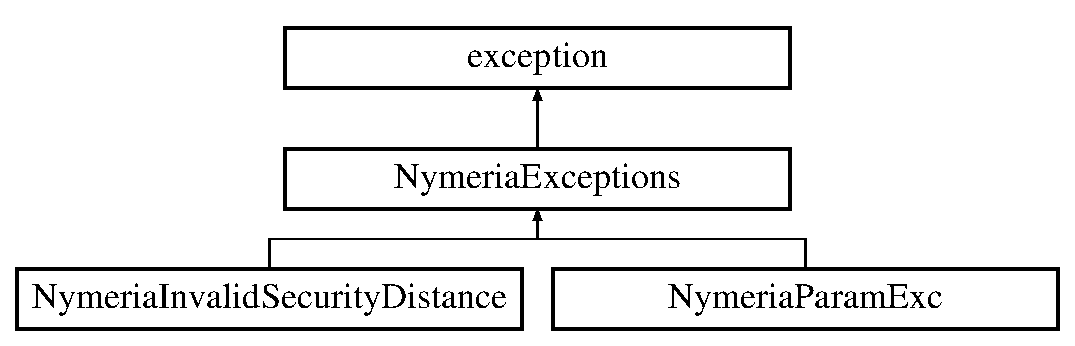
\includegraphics[height=3.000000cm]{class_nymeria_exceptions}
\end{center}
\end{figure}
\subsection*{Public Member Functions}
\begin{DoxyCompactItemize}
\item 
\hyperlink{class_nymeria_exceptions_a2ffc37214bfd0d77123c81e4d11f05c3}{Nymeria\+Exceptions} (string msg)
\begin{DoxyCompactList}\small\item\em Definition of the class \hyperlink{class_nymeria_exceptions}{Nymeria\+Exceptions}, that defines the base class for all exceptions particular to \hyperlink{class_nymeria}{Nymeria}. \end{DoxyCompactList}\item 
virtual \hyperlink{class_nymeria_exceptions_a3c8a85626f56eeb615907c4125d8d9c3}{$\sim$\+Nymeria\+Exceptions} (void)  throw ()
\item 
virtual const char $\ast$ \hyperlink{class_nymeria_exceptions_ab2330e7001e60ca05b3ed72b616b9c8f}{what} () const   throw ()
\end{DoxyCompactItemize}


\subsection{Detailed Description}
Declaration of the class \hyperlink{class_nymeria_exceptions}{Nymeria\+Exceptions}, that declares the base class for all exceptions particular to \hyperlink{class_nymeria}{Nymeria}. 

\subsection{Constructor \& Destructor Documentation}
\hypertarget{class_nymeria_exceptions_a2ffc37214bfd0d77123c81e4d11f05c3}{}\index{Nymeria\+Exceptions@{Nymeria\+Exceptions}!Nymeria\+Exceptions@{Nymeria\+Exceptions}}
\index{Nymeria\+Exceptions@{Nymeria\+Exceptions}!Nymeria\+Exceptions@{Nymeria\+Exceptions}}
\subsubsection[{Nymeria\+Exceptions}]{\setlength{\rightskip}{0pt plus 5cm}Nymeria\+Exceptions\+::\+Nymeria\+Exceptions (
\begin{DoxyParamCaption}
\item[{string}]{msg}
\end{DoxyParamCaption}
)}\label{class_nymeria_exceptions_a2ffc37214bfd0d77123c81e4d11f05c3}


Definition of the class \hyperlink{class_nymeria_exceptions}{Nymeria\+Exceptions}, that defines the base class for all exceptions particular to \hyperlink{class_nymeria}{Nymeria}. 

\hypertarget{class_nymeria_exceptions_a3c8a85626f56eeb615907c4125d8d9c3}{}\index{Nymeria\+Exceptions@{Nymeria\+Exceptions}!````~Nymeria\+Exceptions@{$\sim$\+Nymeria\+Exceptions}}
\index{````~Nymeria\+Exceptions@{$\sim$\+Nymeria\+Exceptions}!Nymeria\+Exceptions@{Nymeria\+Exceptions}}
\subsubsection[{$\sim$\+Nymeria\+Exceptions}]{\setlength{\rightskip}{0pt plus 5cm}Nymeria\+Exceptions\+::$\sim$\+Nymeria\+Exceptions (
\begin{DoxyParamCaption}
\item[{void}]{}
\end{DoxyParamCaption}
) throw  ) \hspace{0.3cm}{\ttfamily [virtual]}}\label{class_nymeria_exceptions_a3c8a85626f56eeb615907c4125d8d9c3}


\subsection{Member Function Documentation}
\hypertarget{class_nymeria_exceptions_ab2330e7001e60ca05b3ed72b616b9c8f}{}\index{Nymeria\+Exceptions@{Nymeria\+Exceptions}!what@{what}}
\index{what@{what}!Nymeria\+Exceptions@{Nymeria\+Exceptions}}
\subsubsection[{what}]{\setlength{\rightskip}{0pt plus 5cm}const char $\ast$ Nymeria\+Exceptions\+::what (
\begin{DoxyParamCaption}
{}
\end{DoxyParamCaption}
) const throw  ) \hspace{0.3cm}{\ttfamily [virtual]}}\label{class_nymeria_exceptions_ab2330e7001e60ca05b3ed72b616b9c8f}


Reimplemented in \hyperlink{class_nymeria_invalid_security_distance_ad355d93e206f208f9994079da463ef75}{Nymeria\+Invalid\+Security\+Distance}, and \hyperlink{class_nymeria_param_exc_ae286e24a03c91eeb062a50f4e090b757}{Nymeria\+Param\+Exc}.



The documentation for this class was generated from the following files\+:\begin{DoxyCompactItemize}
\item 
include/nymeria\+\_\+ardrone/\hyperlink{_nymeria_exceptions_8h}{Nymeria\+Exceptions.\+h}\item 
src/exception/\hyperlink{_nymeria_exceptions_8cpp}{Nymeria\+Exceptions.\+cpp}\end{DoxyCompactItemize}

\hypertarget{class_nymeria_invalid_security_distance}{}\section{Nymeria\+Invalid\+Security\+Distance Class Reference}
\label{class_nymeria_invalid_security_distance}\index{Nymeria\+Invalid\+Security\+Distance@{Nymeria\+Invalid\+Security\+Distance}}


Declaration of the class \hyperlink{class_nymeria_param_exc}{Nymeria\+Param\+Exc}, that declares the exception thrown when the R\+O\+S parameter requested does not exist or was misspelled.  




{\ttfamily \#include $<$Nymeria\+Invalid\+Security\+Distance.\+h$>$}

Inheritance diagram for Nymeria\+Invalid\+Security\+Distance\+:\begin{figure}[H]
\begin{center}
\leavevmode
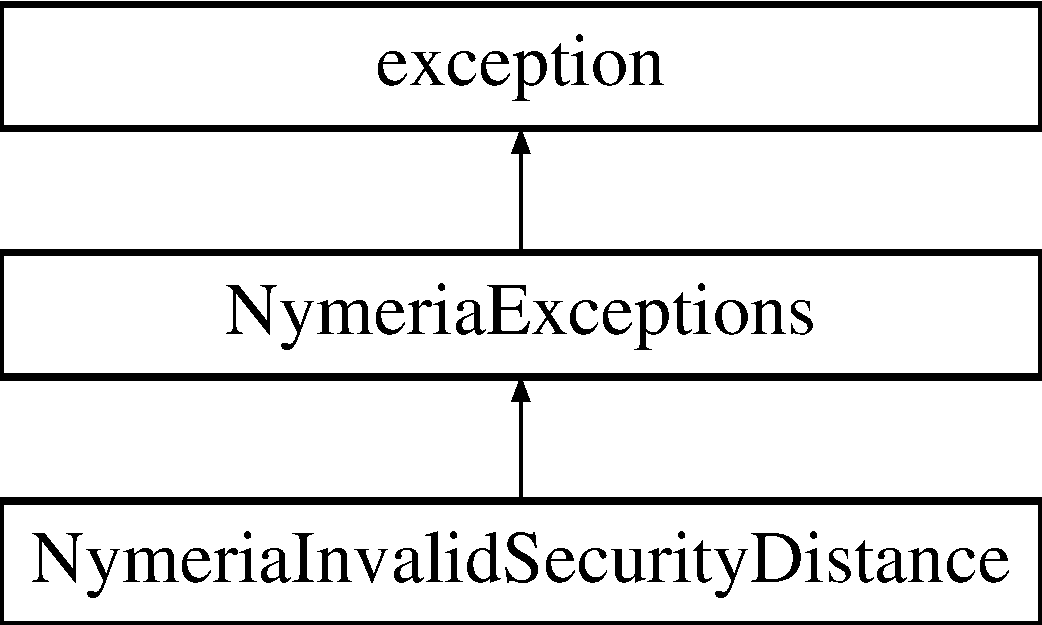
\includegraphics[height=3.000000cm]{class_nymeria_invalid_security_distance}
\end{center}
\end{figure}
\subsection*{Public Member Functions}
\begin{DoxyCompactItemize}
\item 
\hyperlink{class_nymeria_invalid_security_distance_a50c42bc95a0d56f9eafd4d9bbadd96ce}{Nymeria\+Invalid\+Security\+Distance} (void)
\begin{DoxyCompactList}\small\item\em Definition of the class \hyperlink{class_nymeria_invalid_security_distance}{Nymeria\+Invalid\+Security\+Distance}, that defines the exception thrown when the an invalid security distance is entered. \end{DoxyCompactList}\item 
virtual \hyperlink{class_nymeria_invalid_security_distance_ac05209ee7fcc2e62ab8da62afab847d3}{$\sim$\+Nymeria\+Invalid\+Security\+Distance} (void)  throw ()
\item 
virtual const char $\ast$ \hyperlink{class_nymeria_invalid_security_distance_ad355d93e206f208f9994079da463ef75}{what} () const   throw ()
\end{DoxyCompactItemize}


\subsection{Detailed Description}
Declaration of the class \hyperlink{class_nymeria_param_exc}{Nymeria\+Param\+Exc}, that declares the exception thrown when the R\+O\+S parameter requested does not exist or was misspelled. 

\subsection{Constructor \& Destructor Documentation}
\hypertarget{class_nymeria_invalid_security_distance_a50c42bc95a0d56f9eafd4d9bbadd96ce}{}\index{Nymeria\+Invalid\+Security\+Distance@{Nymeria\+Invalid\+Security\+Distance}!Nymeria\+Invalid\+Security\+Distance@{Nymeria\+Invalid\+Security\+Distance}}
\index{Nymeria\+Invalid\+Security\+Distance@{Nymeria\+Invalid\+Security\+Distance}!Nymeria\+Invalid\+Security\+Distance@{Nymeria\+Invalid\+Security\+Distance}}
\subsubsection[{Nymeria\+Invalid\+Security\+Distance}]{\setlength{\rightskip}{0pt plus 5cm}Nymeria\+Invalid\+Security\+Distance\+::\+Nymeria\+Invalid\+Security\+Distance (
\begin{DoxyParamCaption}
\item[{void}]{}
\end{DoxyParamCaption}
)}\label{class_nymeria_invalid_security_distance_a50c42bc95a0d56f9eafd4d9bbadd96ce}


Definition of the class \hyperlink{class_nymeria_invalid_security_distance}{Nymeria\+Invalid\+Security\+Distance}, that defines the exception thrown when the an invalid security distance is entered. 

\hypertarget{class_nymeria_invalid_security_distance_ac05209ee7fcc2e62ab8da62afab847d3}{}\index{Nymeria\+Invalid\+Security\+Distance@{Nymeria\+Invalid\+Security\+Distance}!````~Nymeria\+Invalid\+Security\+Distance@{$\sim$\+Nymeria\+Invalid\+Security\+Distance}}
\index{````~Nymeria\+Invalid\+Security\+Distance@{$\sim$\+Nymeria\+Invalid\+Security\+Distance}!Nymeria\+Invalid\+Security\+Distance@{Nymeria\+Invalid\+Security\+Distance}}
\subsubsection[{$\sim$\+Nymeria\+Invalid\+Security\+Distance}]{\setlength{\rightskip}{0pt plus 5cm}Nymeria\+Invalid\+Security\+Distance\+::$\sim$\+Nymeria\+Invalid\+Security\+Distance (
\begin{DoxyParamCaption}
\item[{void}]{}
\end{DoxyParamCaption}
) throw  ) \hspace{0.3cm}{\ttfamily [virtual]}}\label{class_nymeria_invalid_security_distance_ac05209ee7fcc2e62ab8da62afab847d3}


\subsection{Member Function Documentation}
\hypertarget{class_nymeria_invalid_security_distance_ad355d93e206f208f9994079da463ef75}{}\index{Nymeria\+Invalid\+Security\+Distance@{Nymeria\+Invalid\+Security\+Distance}!what@{what}}
\index{what@{what}!Nymeria\+Invalid\+Security\+Distance@{Nymeria\+Invalid\+Security\+Distance}}
\subsubsection[{what}]{\setlength{\rightskip}{0pt plus 5cm}const char $\ast$ Nymeria\+Invalid\+Security\+Distance\+::what (
\begin{DoxyParamCaption}
{}
\end{DoxyParamCaption}
) const throw  ) \hspace{0.3cm}{\ttfamily [virtual]}}\label{class_nymeria_invalid_security_distance_ad355d93e206f208f9994079da463ef75}


Reimplemented from \hyperlink{class_nymeria_exceptions_ab2330e7001e60ca05b3ed72b616b9c8f}{Nymeria\+Exceptions}.



The documentation for this class was generated from the following files\+:\begin{DoxyCompactItemize}
\item 
include/nymeria\+\_\+ardrone/\hyperlink{_nymeria_invalid_security_distance_8h}{Nymeria\+Invalid\+Security\+Distance.\+h}\item 
src/exception/\hyperlink{_nymeria_invalid_security_distance_8cpp}{Nymeria\+Invalid\+Security\+Distance.\+cpp}\end{DoxyCompactItemize}

\hypertarget{class_nymeria_mutex}{}\section{Nymeria\+Mutex Class Reference}
\label{class_nymeria_mutex}\index{Nymeria\+Mutex@{Nymeria\+Mutex}}


{\ttfamily \#include $<$Nymeria\+Mutex.\+h$>$}

Inheritance diagram for Nymeria\+Mutex\+:\begin{figure}[H]
\begin{center}
\leavevmode
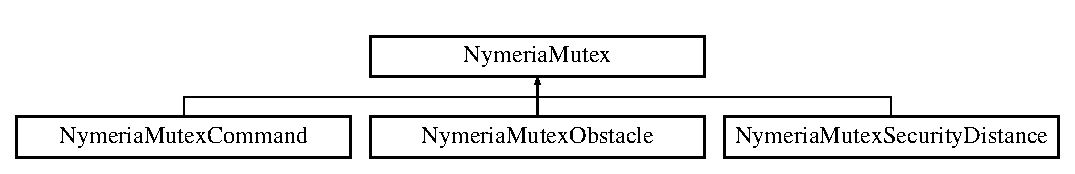
\includegraphics[height=1.895093cm]{class_nymeria_mutex}
\end{center}
\end{figure}
\subsection*{Public Member Functions}
\begin{DoxyCompactItemize}
\item 
\hyperlink{class_nymeria_mutex_a49572f92680c682497e7c557239a39cb}{Nymeria\+Mutex} ()
\end{DoxyCompactItemize}


\subsection{Constructor \& Destructor Documentation}
\hypertarget{class_nymeria_mutex_a49572f92680c682497e7c557239a39cb}{}\index{Nymeria\+Mutex@{Nymeria\+Mutex}!Nymeria\+Mutex@{Nymeria\+Mutex}}
\index{Nymeria\+Mutex@{Nymeria\+Mutex}!Nymeria\+Mutex@{Nymeria\+Mutex}}
\subsubsection[{Nymeria\+Mutex}]{\setlength{\rightskip}{0pt plus 5cm}Nymeria\+Mutex\+::\+Nymeria\+Mutex (
\begin{DoxyParamCaption}
{}
\end{DoxyParamCaption}
)}\label{class_nymeria_mutex_a49572f92680c682497e7c557239a39cb}


The documentation for this class was generated from the following files\+:\begin{DoxyCompactItemize}
\item 
include/nymeria\+\_\+ardrone/\hyperlink{_nymeria_mutex_8h}{Nymeria\+Mutex.\+h}\item 
src/\hyperlink{_nymeria_mutex_8cpp}{Nymeria\+Mutex.\+cpp}\end{DoxyCompactItemize}

\hypertarget{class_nymeria_mutex_command}{}\section{Nymeria\+Mutex\+Command Class Reference}
\label{class_nymeria_mutex_command}\index{Nymeria\+Mutex\+Command@{Nymeria\+Mutex\+Command}}


{\ttfamily \#include $<$Nymeria\+Mutex\+Command.\+h$>$}

Inheritance diagram for Nymeria\+Mutex\+Command\+:\begin{figure}[H]
\begin{center}
\leavevmode
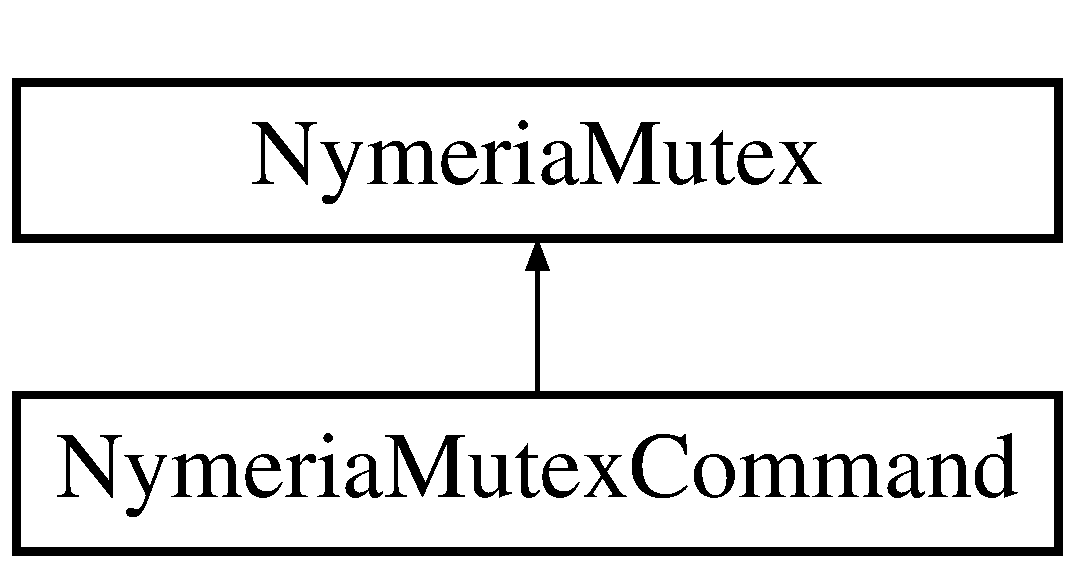
\includegraphics[height=2.000000cm]{class_nymeria_mutex_command}
\end{center}
\end{figure}
\subsection*{Public Member Functions}
\begin{DoxyCompactItemize}
\item 
\hyperlink{class_nymeria_mutex_command_a7d5fc75bb4b2f6106912aba753807f54}{$\sim$\+Nymeria\+Mutex\+Command} ()
\end{DoxyCompactItemize}
\subsection*{Static Public Member Functions}
\begin{DoxyCompactItemize}
\item 
static \hyperlink{class_nymeria_mutex_command}{Nymeria\+Mutex\+Command} $\ast$ \hyperlink{class_nymeria_mutex_command_a3aef40b73394ef9c59c30df348ad760c}{get\+Instance} ()
\item 
static void \hyperlink{class_nymeria_mutex_command_a48016d42ec51705f59c774aa2dc19796}{lock} ()
\item 
static void \hyperlink{class_nymeria_mutex_command_afea66e700a433145efeafd9b8a53df7b}{unlock} ()
\end{DoxyCompactItemize}


\subsection{Constructor \& Destructor Documentation}
\hypertarget{class_nymeria_mutex_command_a7d5fc75bb4b2f6106912aba753807f54}{}\index{Nymeria\+Mutex\+Command@{Nymeria\+Mutex\+Command}!````~Nymeria\+Mutex\+Command@{$\sim$\+Nymeria\+Mutex\+Command}}
\index{````~Nymeria\+Mutex\+Command@{$\sim$\+Nymeria\+Mutex\+Command}!Nymeria\+Mutex\+Command@{Nymeria\+Mutex\+Command}}
\subsubsection[{$\sim$\+Nymeria\+Mutex\+Command}]{\setlength{\rightskip}{0pt plus 5cm}Nymeria\+Mutex\+Command\+::$\sim$\+Nymeria\+Mutex\+Command (
\begin{DoxyParamCaption}
{}
\end{DoxyParamCaption}
)}\label{class_nymeria_mutex_command_a7d5fc75bb4b2f6106912aba753807f54}


\subsection{Member Function Documentation}
\hypertarget{class_nymeria_mutex_command_a3aef40b73394ef9c59c30df348ad760c}{}\index{Nymeria\+Mutex\+Command@{Nymeria\+Mutex\+Command}!get\+Instance@{get\+Instance}}
\index{get\+Instance@{get\+Instance}!Nymeria\+Mutex\+Command@{Nymeria\+Mutex\+Command}}
\subsubsection[{get\+Instance}]{\setlength{\rightskip}{0pt plus 5cm}{\bf Nymeria\+Mutex\+Command} $\ast$ Nymeria\+Mutex\+Command\+::get\+Instance (
\begin{DoxyParamCaption}
{}
\end{DoxyParamCaption}
)\hspace{0.3cm}{\ttfamily [static]}}\label{class_nymeria_mutex_command_a3aef40b73394ef9c59c30df348ad760c}
\hypertarget{class_nymeria_mutex_command_a48016d42ec51705f59c774aa2dc19796}{}\index{Nymeria\+Mutex\+Command@{Nymeria\+Mutex\+Command}!lock@{lock}}
\index{lock@{lock}!Nymeria\+Mutex\+Command@{Nymeria\+Mutex\+Command}}
\subsubsection[{lock}]{\setlength{\rightskip}{0pt plus 5cm}void Nymeria\+Mutex\+Command\+::lock (
\begin{DoxyParamCaption}
{}
\end{DoxyParamCaption}
)\hspace{0.3cm}{\ttfamily [static]}}\label{class_nymeria_mutex_command_a48016d42ec51705f59c774aa2dc19796}
\hypertarget{class_nymeria_mutex_command_afea66e700a433145efeafd9b8a53df7b}{}\index{Nymeria\+Mutex\+Command@{Nymeria\+Mutex\+Command}!unlock@{unlock}}
\index{unlock@{unlock}!Nymeria\+Mutex\+Command@{Nymeria\+Mutex\+Command}}
\subsubsection[{unlock}]{\setlength{\rightskip}{0pt plus 5cm}void Nymeria\+Mutex\+Command\+::unlock (
\begin{DoxyParamCaption}
{}
\end{DoxyParamCaption}
)\hspace{0.3cm}{\ttfamily [static]}}\label{class_nymeria_mutex_command_afea66e700a433145efeafd9b8a53df7b}


The documentation for this class was generated from the following files\+:\begin{DoxyCompactItemize}
\item 
include/nymeria\+\_\+ardrone/\hyperlink{_nymeria_mutex_command_8h}{Nymeria\+Mutex\+Command.\+h}\item 
src/\hyperlink{_nymeria_mutex_command_8cpp}{Nymeria\+Mutex\+Command.\+cpp}\end{DoxyCompactItemize}

\hypertarget{class_nymeria_mutex_obstacle}{}\section{Nymeria\+Mutex\+Obstacle Class Reference}
\label{class_nymeria_mutex_obstacle}\index{Nymeria\+Mutex\+Obstacle@{Nymeria\+Mutex\+Obstacle}}


{\ttfamily \#include $<$Nymeria\+Mutex\+Obstacle.\+h$>$}

Inheritance diagram for Nymeria\+Mutex\+Obstacle\+:\begin{figure}[H]
\begin{center}
\leavevmode
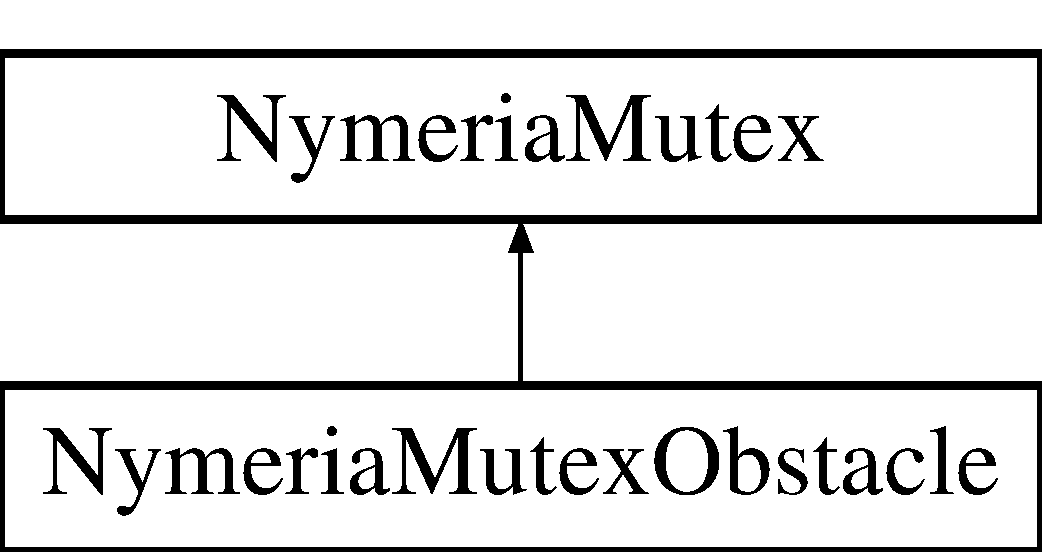
\includegraphics[height=2.000000cm]{class_nymeria_mutex_obstacle}
\end{center}
\end{figure}
\subsection*{Public Member Functions}
\begin{DoxyCompactItemize}
\item 
\hyperlink{class_nymeria_mutex_obstacle_a633b42cd43d18923e7dbe0430fc0bf8c}{$\sim$\+Nymeria\+Mutex\+Obstacle} ()
\end{DoxyCompactItemize}
\subsection*{Static Public Member Functions}
\begin{DoxyCompactItemize}
\item 
static \hyperlink{class_nymeria_mutex_obstacle}{Nymeria\+Mutex\+Obstacle} $\ast$ \hyperlink{class_nymeria_mutex_obstacle_a781305cfbe891eaf547c9d023b42d272}{get\+Instance} ()
\item 
static void \hyperlink{class_nymeria_mutex_obstacle_ac9c77e3c39a6037aaf356d9d82460a40}{lock} ()
\item 
static void \hyperlink{class_nymeria_mutex_obstacle_ae10b2974844ac973a692be10eeaddf79}{unlock} ()
\end{DoxyCompactItemize}


\subsection{Constructor \& Destructor Documentation}
\hypertarget{class_nymeria_mutex_obstacle_a633b42cd43d18923e7dbe0430fc0bf8c}{}\index{Nymeria\+Mutex\+Obstacle@{Nymeria\+Mutex\+Obstacle}!````~Nymeria\+Mutex\+Obstacle@{$\sim$\+Nymeria\+Mutex\+Obstacle}}
\index{````~Nymeria\+Mutex\+Obstacle@{$\sim$\+Nymeria\+Mutex\+Obstacle}!Nymeria\+Mutex\+Obstacle@{Nymeria\+Mutex\+Obstacle}}
\subsubsection[{$\sim$\+Nymeria\+Mutex\+Obstacle}]{\setlength{\rightskip}{0pt plus 5cm}Nymeria\+Mutex\+Obstacle\+::$\sim$\+Nymeria\+Mutex\+Obstacle (
\begin{DoxyParamCaption}
{}
\end{DoxyParamCaption}
)}\label{class_nymeria_mutex_obstacle_a633b42cd43d18923e7dbe0430fc0bf8c}


\subsection{Member Function Documentation}
\hypertarget{class_nymeria_mutex_obstacle_a781305cfbe891eaf547c9d023b42d272}{}\index{Nymeria\+Mutex\+Obstacle@{Nymeria\+Mutex\+Obstacle}!get\+Instance@{get\+Instance}}
\index{get\+Instance@{get\+Instance}!Nymeria\+Mutex\+Obstacle@{Nymeria\+Mutex\+Obstacle}}
\subsubsection[{get\+Instance}]{\setlength{\rightskip}{0pt plus 5cm}{\bf Nymeria\+Mutex\+Obstacle} $\ast$ Nymeria\+Mutex\+Obstacle\+::get\+Instance (
\begin{DoxyParamCaption}
{}
\end{DoxyParamCaption}
)\hspace{0.3cm}{\ttfamily [static]}}\label{class_nymeria_mutex_obstacle_a781305cfbe891eaf547c9d023b42d272}
\hypertarget{class_nymeria_mutex_obstacle_ac9c77e3c39a6037aaf356d9d82460a40}{}\index{Nymeria\+Mutex\+Obstacle@{Nymeria\+Mutex\+Obstacle}!lock@{lock}}
\index{lock@{lock}!Nymeria\+Mutex\+Obstacle@{Nymeria\+Mutex\+Obstacle}}
\subsubsection[{lock}]{\setlength{\rightskip}{0pt plus 5cm}void Nymeria\+Mutex\+Obstacle\+::lock (
\begin{DoxyParamCaption}
{}
\end{DoxyParamCaption}
)\hspace{0.3cm}{\ttfamily [static]}}\label{class_nymeria_mutex_obstacle_ac9c77e3c39a6037aaf356d9d82460a40}
\hypertarget{class_nymeria_mutex_obstacle_ae10b2974844ac973a692be10eeaddf79}{}\index{Nymeria\+Mutex\+Obstacle@{Nymeria\+Mutex\+Obstacle}!unlock@{unlock}}
\index{unlock@{unlock}!Nymeria\+Mutex\+Obstacle@{Nymeria\+Mutex\+Obstacle}}
\subsubsection[{unlock}]{\setlength{\rightskip}{0pt plus 5cm}void Nymeria\+Mutex\+Obstacle\+::unlock (
\begin{DoxyParamCaption}
{}
\end{DoxyParamCaption}
)\hspace{0.3cm}{\ttfamily [static]}}\label{class_nymeria_mutex_obstacle_ae10b2974844ac973a692be10eeaddf79}


The documentation for this class was generated from the following files\+:\begin{DoxyCompactItemize}
\item 
include/nymeria\+\_\+ardrone/\hyperlink{_nymeria_mutex_obstacle_8h}{Nymeria\+Mutex\+Obstacle.\+h}\item 
src/\hyperlink{_nymeria_mutex_obstacle_8cpp}{Nymeria\+Mutex\+Obstacle.\+cpp}\end{DoxyCompactItemize}

\hypertarget{class_nymeria_mutex_security_distance}{}\section{Nymeria\+Mutex\+Security\+Distance Class Reference}
\label{class_nymeria_mutex_security_distance}\index{Nymeria\+Mutex\+Security\+Distance@{Nymeria\+Mutex\+Security\+Distance}}


{\ttfamily \#include $<$Nymeria\+Mutex\+Security\+Distance.\+h$>$}

Inheritance diagram for Nymeria\+Mutex\+Security\+Distance\+:\begin{figure}[H]
\begin{center}
\leavevmode
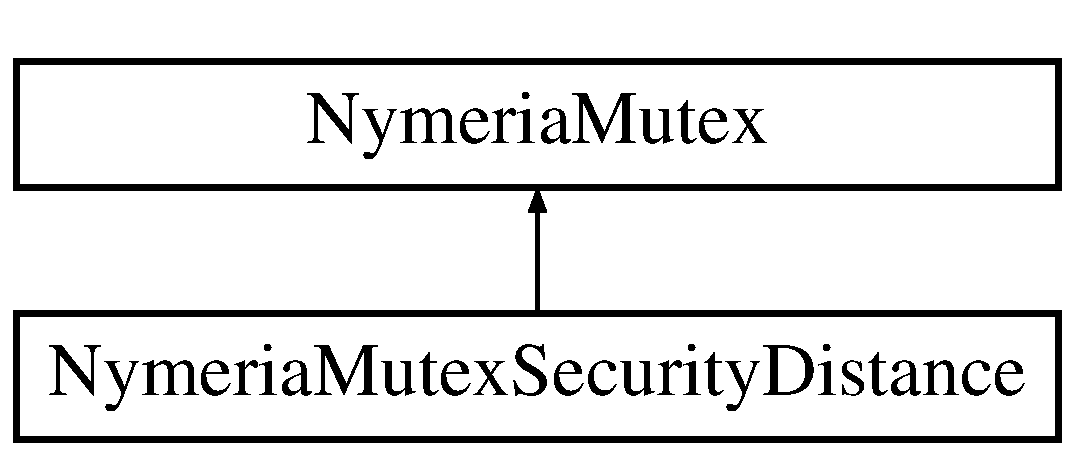
\includegraphics[height=2.000000cm]{class_nymeria_mutex_security_distance}
\end{center}
\end{figure}
\subsection*{Public Member Functions}
\begin{DoxyCompactItemize}
\item 
\hyperlink{class_nymeria_mutex_security_distance_a8dcc9a0342a2520db12cd458c15f04c5}{$\sim$\+Nymeria\+Mutex\+Security\+Distance} ()
\end{DoxyCompactItemize}
\subsection*{Static Public Member Functions}
\begin{DoxyCompactItemize}
\item 
static \hyperlink{class_nymeria_mutex_security_distance}{Nymeria\+Mutex\+Security\+Distance} $\ast$ \hyperlink{class_nymeria_mutex_security_distance_a7de1c0314682fcdecf8e882eab57362b}{get\+Instance} ()
\item 
static void \hyperlink{class_nymeria_mutex_security_distance_a983390ed9dcef9b62c3df39f47e5bbe7}{lock} ()
\item 
static void \hyperlink{class_nymeria_mutex_security_distance_a13d05cc109b0198a05091f0e2b108db5}{unlock} ()
\end{DoxyCompactItemize}


\subsection{Constructor \& Destructor Documentation}
\hypertarget{class_nymeria_mutex_security_distance_a8dcc9a0342a2520db12cd458c15f04c5}{}\index{Nymeria\+Mutex\+Security\+Distance@{Nymeria\+Mutex\+Security\+Distance}!````~Nymeria\+Mutex\+Security\+Distance@{$\sim$\+Nymeria\+Mutex\+Security\+Distance}}
\index{````~Nymeria\+Mutex\+Security\+Distance@{$\sim$\+Nymeria\+Mutex\+Security\+Distance}!Nymeria\+Mutex\+Security\+Distance@{Nymeria\+Mutex\+Security\+Distance}}
\subsubsection[{$\sim$\+Nymeria\+Mutex\+Security\+Distance}]{\setlength{\rightskip}{0pt plus 5cm}Nymeria\+Mutex\+Security\+Distance\+::$\sim$\+Nymeria\+Mutex\+Security\+Distance (
\begin{DoxyParamCaption}
{}
\end{DoxyParamCaption}
)}\label{class_nymeria_mutex_security_distance_a8dcc9a0342a2520db12cd458c15f04c5}


\subsection{Member Function Documentation}
\hypertarget{class_nymeria_mutex_security_distance_a7de1c0314682fcdecf8e882eab57362b}{}\index{Nymeria\+Mutex\+Security\+Distance@{Nymeria\+Mutex\+Security\+Distance}!get\+Instance@{get\+Instance}}
\index{get\+Instance@{get\+Instance}!Nymeria\+Mutex\+Security\+Distance@{Nymeria\+Mutex\+Security\+Distance}}
\subsubsection[{get\+Instance}]{\setlength{\rightskip}{0pt plus 5cm}{\bf Nymeria\+Mutex\+Security\+Distance} $\ast$ Nymeria\+Mutex\+Security\+Distance\+::get\+Instance (
\begin{DoxyParamCaption}
{}
\end{DoxyParamCaption}
)\hspace{0.3cm}{\ttfamily [static]}}\label{class_nymeria_mutex_security_distance_a7de1c0314682fcdecf8e882eab57362b}
\hypertarget{class_nymeria_mutex_security_distance_a983390ed9dcef9b62c3df39f47e5bbe7}{}\index{Nymeria\+Mutex\+Security\+Distance@{Nymeria\+Mutex\+Security\+Distance}!lock@{lock}}
\index{lock@{lock}!Nymeria\+Mutex\+Security\+Distance@{Nymeria\+Mutex\+Security\+Distance}}
\subsubsection[{lock}]{\setlength{\rightskip}{0pt plus 5cm}void Nymeria\+Mutex\+Security\+Distance\+::lock (
\begin{DoxyParamCaption}
{}
\end{DoxyParamCaption}
)\hspace{0.3cm}{\ttfamily [static]}}\label{class_nymeria_mutex_security_distance_a983390ed9dcef9b62c3df39f47e5bbe7}
\hypertarget{class_nymeria_mutex_security_distance_a13d05cc109b0198a05091f0e2b108db5}{}\index{Nymeria\+Mutex\+Security\+Distance@{Nymeria\+Mutex\+Security\+Distance}!unlock@{unlock}}
\index{unlock@{unlock}!Nymeria\+Mutex\+Security\+Distance@{Nymeria\+Mutex\+Security\+Distance}}
\subsubsection[{unlock}]{\setlength{\rightskip}{0pt plus 5cm}void Nymeria\+Mutex\+Security\+Distance\+::unlock (
\begin{DoxyParamCaption}
{}
\end{DoxyParamCaption}
)\hspace{0.3cm}{\ttfamily [static]}}\label{class_nymeria_mutex_security_distance_a13d05cc109b0198a05091f0e2b108db5}


The documentation for this class was generated from the following files\+:\begin{DoxyCompactItemize}
\item 
include/nymeria\+\_\+ardrone/\hyperlink{_nymeria_mutex_security_distance_8h}{Nymeria\+Mutex\+Security\+Distance.\+h}\item 
src/\hyperlink{_nymeria_mutex_security_distance_8cpp}{Nymeria\+Mutex\+Security\+Distance.\+cpp}\end{DoxyCompactItemize}

\hypertarget{class_nymeria_param_exc}{}\section{Nymeria\+Param\+Exc Class Reference}
\label{class_nymeria_param_exc}\index{Nymeria\+Param\+Exc@{Nymeria\+Param\+Exc}}


Declaration of the class \hyperlink{class_nymeria_param_exc}{Nymeria\+Param\+Exc}, that declares the exception thrown when the R\+O\+S parameter requested does not exist or was misspelled.  




{\ttfamily \#include $<$Nymeria\+Param\+Exc.\+h$>$}

Inheritance diagram for Nymeria\+Param\+Exc\+:\begin{figure}[H]
\begin{center}
\leavevmode
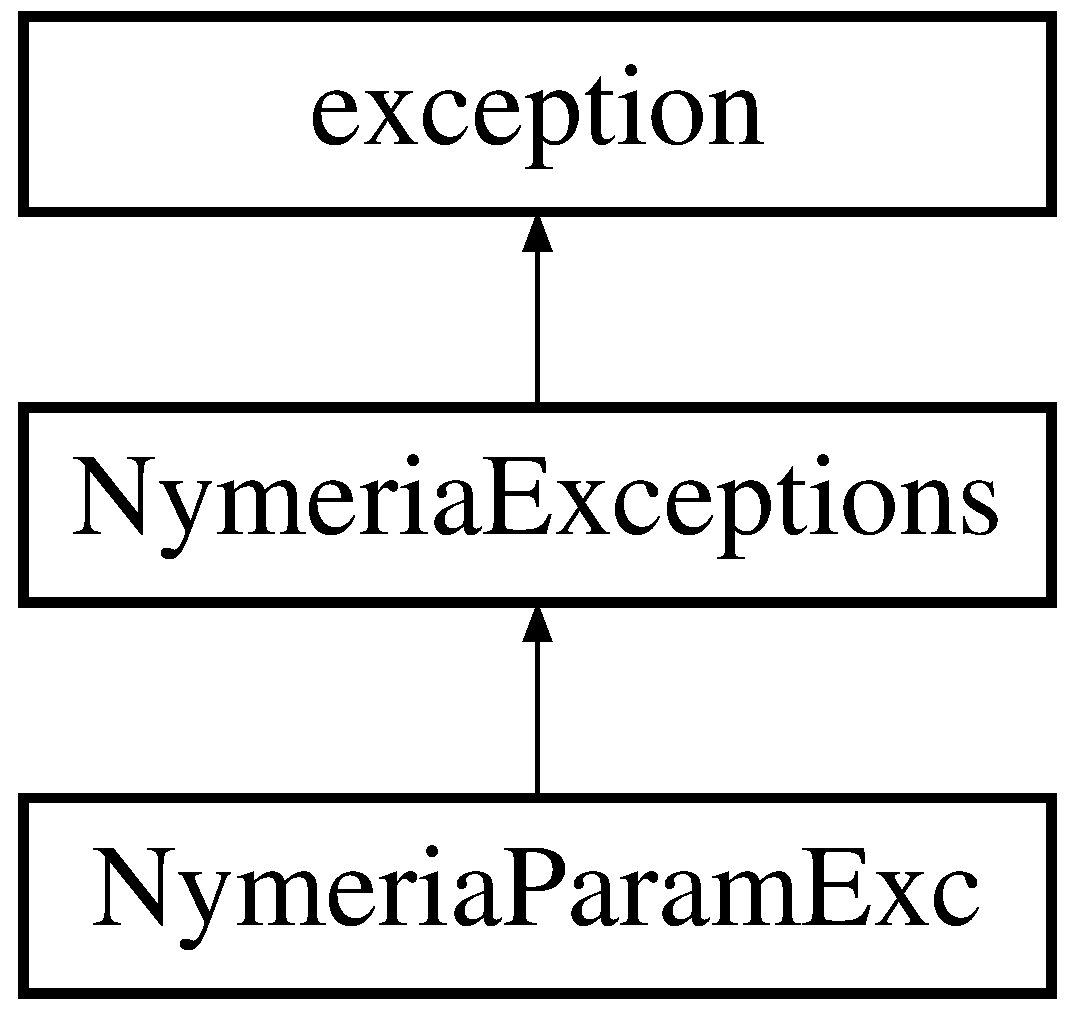
\includegraphics[height=3.000000cm]{class_nymeria_param_exc}
\end{center}
\end{figure}
\subsection*{Public Member Functions}
\begin{DoxyCompactItemize}
\item 
\hyperlink{class_nymeria_param_exc_a253c3cfe3e927036a1043836394cb6fe}{Nymeria\+Param\+Exc} (string msg=\char`\"{}\char`\"{})
\begin{DoxyCompactList}\small\item\em Definition of the class \hyperlink{class_nymeria_param_exc}{Nymeria\+Param\+Exc}, that defines the exception thrown when the R\+O\+S parameter requested does not exist or was misspelled. \end{DoxyCompactList}\item 
virtual \hyperlink{class_nymeria_param_exc_af6d407354b2432ef7a9e0c504802f955}{$\sim$\+Nymeria\+Param\+Exc} (void)  throw ()
\item 
virtual const char $\ast$ \hyperlink{class_nymeria_param_exc_ae286e24a03c91eeb062a50f4e090b757}{what} () const   throw ()
\end{DoxyCompactItemize}


\subsection{Detailed Description}
Declaration of the class \hyperlink{class_nymeria_param_exc}{Nymeria\+Param\+Exc}, that declares the exception thrown when the R\+O\+S parameter requested does not exist or was misspelled. 

\subsection{Constructor \& Destructor Documentation}
\hypertarget{class_nymeria_param_exc_a253c3cfe3e927036a1043836394cb6fe}{}\index{Nymeria\+Param\+Exc@{Nymeria\+Param\+Exc}!Nymeria\+Param\+Exc@{Nymeria\+Param\+Exc}}
\index{Nymeria\+Param\+Exc@{Nymeria\+Param\+Exc}!Nymeria\+Param\+Exc@{Nymeria\+Param\+Exc}}
\subsubsection[{Nymeria\+Param\+Exc}]{\setlength{\rightskip}{0pt plus 5cm}Nymeria\+Param\+Exc\+::\+Nymeria\+Param\+Exc (
\begin{DoxyParamCaption}
\item[{string}]{msg = {\ttfamily \char`\"{}\char`\"{}}}
\end{DoxyParamCaption}
)}\label{class_nymeria_param_exc_a253c3cfe3e927036a1043836394cb6fe}


Definition of the class \hyperlink{class_nymeria_param_exc}{Nymeria\+Param\+Exc}, that defines the exception thrown when the R\+O\+S parameter requested does not exist or was misspelled. 

\hypertarget{class_nymeria_param_exc_af6d407354b2432ef7a9e0c504802f955}{}\index{Nymeria\+Param\+Exc@{Nymeria\+Param\+Exc}!````~Nymeria\+Param\+Exc@{$\sim$\+Nymeria\+Param\+Exc}}
\index{````~Nymeria\+Param\+Exc@{$\sim$\+Nymeria\+Param\+Exc}!Nymeria\+Param\+Exc@{Nymeria\+Param\+Exc}}
\subsubsection[{$\sim$\+Nymeria\+Param\+Exc}]{\setlength{\rightskip}{0pt plus 5cm}Nymeria\+Param\+Exc\+::$\sim$\+Nymeria\+Param\+Exc (
\begin{DoxyParamCaption}
\item[{void}]{}
\end{DoxyParamCaption}
) throw  ) \hspace{0.3cm}{\ttfamily [virtual]}}\label{class_nymeria_param_exc_af6d407354b2432ef7a9e0c504802f955}


\subsection{Member Function Documentation}
\hypertarget{class_nymeria_param_exc_ae286e24a03c91eeb062a50f4e090b757}{}\index{Nymeria\+Param\+Exc@{Nymeria\+Param\+Exc}!what@{what}}
\index{what@{what}!Nymeria\+Param\+Exc@{Nymeria\+Param\+Exc}}
\subsubsection[{what}]{\setlength{\rightskip}{0pt plus 5cm}const char $\ast$ Nymeria\+Param\+Exc\+::what (
\begin{DoxyParamCaption}
{}
\end{DoxyParamCaption}
) const throw  ) \hspace{0.3cm}{\ttfamily [virtual]}}\label{class_nymeria_param_exc_ae286e24a03c91eeb062a50f4e090b757}


Reimplemented from \hyperlink{class_nymeria_exceptions_ab2330e7001e60ca05b3ed72b616b9c8f}{Nymeria\+Exceptions}.



The documentation for this class was generated from the following files\+:\begin{DoxyCompactItemize}
\item 
include/nymeria\+\_\+ardrone/\hyperlink{_nymeria_param_exc_8h}{Nymeria\+Param\+Exc.\+h}\item 
src/exception/\hyperlink{_nymeria_param_exc_8cpp}{Nymeria\+Param\+Exc.\+cpp}\end{DoxyCompactItemize}

\chapter{File Documentation}
\hypertarget{_nymeria_8h}{}\section{include/nymeria\+\_\+ardrone/\+Nymeria.h File Reference}
\label{_nymeria_8h}\index{include/nymeria\+\_\+ardrone/\+Nymeria.\+h@{include/nymeria\+\_\+ardrone/\+Nymeria.\+h}}
{\ttfamily \#include \char`\"{}ros/ros.\+h\char`\"{}}\\*
{\ttfamily \#include \char`\"{}std\+\_\+msgs/\+Empty.\+h\char`\"{}}\\*
{\ttfamily \#include \char`\"{}geometry\+\_\+msgs/\+Twist.\+h\char`\"{}}\\*
{\ttfamily \#include \char`\"{}std\+\_\+msgs/\+U\+Int8.\+h\char`\"{}}\\*
{\ttfamily \#include \char`\"{}std\+\_\+msgs/\+String.\+h\char`\"{}}\\*
{\ttfamily \#include $<$ardrone\+\_\+autonomy/\+Navdata.\+h$>$}\\*
{\ttfamily \#include $<$nymeria\+\_\+ardrone/\+Nymeria\+Constants.\+h$>$}\\*
{\ttfamily \#include $<$nymeria\+\_\+ardrone/\+Controller.\+h$>$}\\*
\subsection*{Classes}
\begin{DoxyCompactItemize}
\item 
class \hyperlink{class_nymeria}{Nymeria}
\begin{DoxyCompactList}\small\item\em Definitions of the class \hyperlink{class_nymeria}{Nymeria}, that declares all functionalities in order to allow for drone navigation with obstacle detection and avoidance. \end{DoxyCompactList}\end{DoxyCompactItemize}

\hypertarget{_nymeria_check_obstacle_8h}{}\section{include/nymeria\+\_\+ardrone/\+Nymeria\+Check\+Obstacle.h File Reference}
\label{_nymeria_check_obstacle_8h}\index{include/nymeria\+\_\+ardrone/\+Nymeria\+Check\+Obstacle.\+h@{include/nymeria\+\_\+ardrone/\+Nymeria\+Check\+Obstacle.\+h}}
{\ttfamily \#include \char`\"{}ros/ros.\+h\char`\"{}}\\*
{\ttfamily \#include $<$ardrone\+\_\+autonomy/\+Navdata.\+h$>$}\\*
\subsection*{Classes}
\begin{DoxyCompactItemize}
\item 
class \hyperlink{class_nymeria_check_obstacle}{Nymeria\+Check\+Obstacle}
\end{DoxyCompactItemize}
\subsection*{Functions}
\begin{DoxyCompactItemize}
\item 
void \hyperlink{_nymeria_check_obstacle_8h_a56de6864332e5218374e99a4283252c3}{state\+Drone\+Callback} (const ardrone\+\_\+autonomy\+::\+Navdata \&data)
\begin{DoxyCompactList}\small\item\em callback function for the subscriber sub\+\_\+navdata gets the pitch of the drone and its state \end{DoxyCompactList}\end{DoxyCompactItemize}


\subsection{Function Documentation}
\hypertarget{_nymeria_check_obstacle_8h_a56de6864332e5218374e99a4283252c3}{}\index{Nymeria\+Check\+Obstacle.\+h@{Nymeria\+Check\+Obstacle.\+h}!state\+Drone\+Callback@{state\+Drone\+Callback}}
\index{state\+Drone\+Callback@{state\+Drone\+Callback}!Nymeria\+Check\+Obstacle.\+h@{Nymeria\+Check\+Obstacle.\+h}}
\subsubsection[{state\+Drone\+Callback}]{\setlength{\rightskip}{0pt plus 5cm}void state\+Drone\+Callback (
\begin{DoxyParamCaption}
\item[{const ardrone\+\_\+autonomy\+::\+Navdata \&}]{data}
\end{DoxyParamCaption}
)}\label{_nymeria_check_obstacle_8h_a56de6864332e5218374e99a4283252c3}


callback function for the subscriber sub\+\_\+navdata gets the pitch of the drone and its state 


\begin{DoxyParams}{Parameters}
{\em data} & variable where the value is stored, must be const \\
\hline
\end{DoxyParams}

\hypertarget{_nymeria_constants_8h}{}\section{include/nymeria\+\_\+ardrone/\+Nymeria\+Constants.h File Reference}
\label{_nymeria_constants_8h}\index{include/nymeria\+\_\+ardrone/\+Nymeria\+Constants.\+h@{include/nymeria\+\_\+ardrone/\+Nymeria\+Constants.\+h}}
\subsection*{Classes}
\begin{DoxyCompactItemize}
\item 
class \hyperlink{class_nymeria_constants}{Nymeria\+Constants}
\begin{DoxyCompactList}\small\item\em Declaration of the class \hyperlink{class_nymeria_constants}{Nymeria\+Constants}, that defines all constants necessary to define both commands and states of the drone and obstacles. \end{DoxyCompactList}\end{DoxyCompactItemize}

\hypertarget{_nymeria_exceptions_8h}{}\section{include/nymeria\+\_\+ardrone/\+Nymeria\+Exceptions.h File Reference}
\label{_nymeria_exceptions_8h}\index{include/nymeria\+\_\+ardrone/\+Nymeria\+Exceptions.\+h@{include/nymeria\+\_\+ardrone/\+Nymeria\+Exceptions.\+h}}
{\ttfamily \#include $<$exception$>$}\\*
{\ttfamily \#include $<$string$>$}\\*
\subsection*{Classes}
\begin{DoxyCompactItemize}
\item 
class \hyperlink{class_nymeria_exceptions}{Nymeria\+Exceptions}
\begin{DoxyCompactList}\small\item\em Declaration of the class \hyperlink{class_nymeria_exceptions}{Nymeria\+Exceptions}, that declares the base class for all exceptions particular to \hyperlink{class_nymeria}{Nymeria}. \end{DoxyCompactList}\end{DoxyCompactItemize}

\hypertarget{_nymeria_invalid_security_distance_8h}{}\section{include/nymeria\+\_\+ardrone/\+Nymeria\+Invalid\+Security\+Distance.h File Reference}
\label{_nymeria_invalid_security_distance_8h}\index{include/nymeria\+\_\+ardrone/\+Nymeria\+Invalid\+Security\+Distance.\+h@{include/nymeria\+\_\+ardrone/\+Nymeria\+Invalid\+Security\+Distance.\+h}}
{\ttfamily \#include $<$nymeria\+\_\+ardrone/\+Nymeria\+Exceptions.\+h$>$}\\*
\subsection*{Classes}
\begin{DoxyCompactItemize}
\item 
class \hyperlink{class_nymeria_invalid_security_distance}{Nymeria\+Invalid\+Security\+Distance}
\begin{DoxyCompactList}\small\item\em Declaration of the class \hyperlink{class_nymeria_param_exc}{Nymeria\+Param\+Exc}, that declares the exception thrown when the R\+O\+S parameter requested does not exist or was misspelled. \end{DoxyCompactList}\end{DoxyCompactItemize}

\hypertarget{_nymeria_mutex_8h}{}\section{include/nymeria\+\_\+ardrone/\+Nymeria\+Mutex.h File Reference}
\label{_nymeria_mutex_8h}\index{include/nymeria\+\_\+ardrone/\+Nymeria\+Mutex.\+h@{include/nymeria\+\_\+ardrone/\+Nymeria\+Mutex.\+h}}
\subsection*{Classes}
\begin{DoxyCompactItemize}
\item 
class \hyperlink{class_nymeria_mutex}{Nymeria\+Mutex}
\end{DoxyCompactItemize}

\hypertarget{_nymeria_mutex_command_8h}{}\section{include/nymeria\+\_\+ardrone/\+Nymeria\+Mutex\+Command.h File Reference}
\label{_nymeria_mutex_command_8h}\index{include/nymeria\+\_\+ardrone/\+Nymeria\+Mutex\+Command.\+h@{include/nymeria\+\_\+ardrone/\+Nymeria\+Mutex\+Command.\+h}}
{\ttfamily \#include $<$nymeria\+\_\+ardrone/\+Nymeria\+Mutex.\+h$>$}\\*
\subsection*{Classes}
\begin{DoxyCompactItemize}
\item 
class \hyperlink{class_nymeria_mutex_command}{Nymeria\+Mutex\+Command}
\end{DoxyCompactItemize}

\hypertarget{_nymeria_mutex_obstacle_8h}{}\section{include/nymeria\+\_\+ardrone/\+Nymeria\+Mutex\+Obstacle.h File Reference}
\label{_nymeria_mutex_obstacle_8h}\index{include/nymeria\+\_\+ardrone/\+Nymeria\+Mutex\+Obstacle.\+h@{include/nymeria\+\_\+ardrone/\+Nymeria\+Mutex\+Obstacle.\+h}}
{\ttfamily \#include $<$nymeria\+\_\+ardrone/\+Nymeria\+Mutex.\+h$>$}\\*
\subsection*{Classes}
\begin{DoxyCompactItemize}
\item 
class \hyperlink{class_nymeria_mutex_obstacle}{Nymeria\+Mutex\+Obstacle}
\end{DoxyCompactItemize}

\hypertarget{_nymeria_mutex_security_distance_8h}{}\section{include/nymeria\+\_\+ardrone/\+Nymeria\+Mutex\+Security\+Distance.h File Reference}
\label{_nymeria_mutex_security_distance_8h}\index{include/nymeria\+\_\+ardrone/\+Nymeria\+Mutex\+Security\+Distance.\+h@{include/nymeria\+\_\+ardrone/\+Nymeria\+Mutex\+Security\+Distance.\+h}}
{\ttfamily \#include $<$nymeria\+\_\+ardrone/\+Nymeria\+Mutex.\+h$>$}\\*
\subsection*{Classes}
\begin{DoxyCompactItemize}
\item 
class \hyperlink{class_nymeria_mutex_security_distance}{Nymeria\+Mutex\+Security\+Distance}
\end{DoxyCompactItemize}

\hypertarget{_nymeria_param_exc_8h}{}\section{include/nymeria\+\_\+ardrone/\+Nymeria\+Param\+Exc.h File Reference}
\label{_nymeria_param_exc_8h}\index{include/nymeria\+\_\+ardrone/\+Nymeria\+Param\+Exc.\+h@{include/nymeria\+\_\+ardrone/\+Nymeria\+Param\+Exc.\+h}}
{\ttfamily \#include $<$nymeria\+\_\+ardrone/\+Nymeria\+Exceptions.\+h$>$}\\*
\subsection*{Classes}
\begin{DoxyCompactItemize}
\item 
class \hyperlink{class_nymeria_param_exc}{Nymeria\+Param\+Exc}
\begin{DoxyCompactList}\small\item\em Declaration of the class \hyperlink{class_nymeria_param_exc}{Nymeria\+Param\+Exc}, that declares the exception thrown when the R\+O\+S parameter requested does not exist or was misspelled. \end{DoxyCompactList}\end{DoxyCompactItemize}

\hypertarget{_r_e_a_d_m_e_8md}{}\section{R\+E\+A\+D\+M\+E.\+md File Reference}
\label{_r_e_a_d_m_e_8md}\index{R\+E\+A\+D\+M\+E.\+md@{R\+E\+A\+D\+M\+E.\+md}}

\hypertarget{_nymeria_exceptions_8cpp}{}\section{src/exception/\+Nymeria\+Exceptions.cpp File Reference}
\label{_nymeria_exceptions_8cpp}\index{src/exception/\+Nymeria\+Exceptions.\+cpp@{src/exception/\+Nymeria\+Exceptions.\+cpp}}
{\ttfamily \#include $<$nymeria\+\_\+ardrone/\+Nymeria\+Exceptions.\+h$>$}\\*

\hypertarget{_nymeria_invalid_security_distance_8cpp}{}\section{src/exception/\+Nymeria\+Invalid\+Security\+Distance.cpp File Reference}
\label{_nymeria_invalid_security_distance_8cpp}\index{src/exception/\+Nymeria\+Invalid\+Security\+Distance.\+cpp@{src/exception/\+Nymeria\+Invalid\+Security\+Distance.\+cpp}}
{\ttfamily \#include $<$nymeria\+\_\+ardrone/\+Nymeria\+Invalid\+Security\+Distance.\+h$>$}\\*

\hypertarget{_nymeria_param_exc_8cpp}{}\section{src/exception/\+Nymeria\+Param\+Exc.cpp File Reference}
\label{_nymeria_param_exc_8cpp}\index{src/exception/\+Nymeria\+Param\+Exc.\+cpp@{src/exception/\+Nymeria\+Param\+Exc.\+cpp}}
{\ttfamily \#include $<$nymeria\+\_\+ardrone/\+Nymeria\+Param\+Exc.\+h$>$}\\*

\hypertarget{_nymeria_8cpp}{}\section{src/\+Nymeria.cpp File Reference}
\label{_nymeria_8cpp}\index{src/\+Nymeria.\+cpp@{src/\+Nymeria.\+cpp}}
{\ttfamily \#include $<$nymeria\+\_\+ardrone/\+Nymeria.\+h$>$}\\*
{\ttfamily \#include $<$nymeria\+\_\+ardrone/\+Nymeria\+Param\+Exc.\+h$>$}\\*
{\ttfamily \#include $<$nymeria\+\_\+ardrone/\+Nymeria\+Invalid\+Security\+Distance.\+h$>$}\\*
{\ttfamily \#include $<$nymeria\+\_\+ardrone/\+Nymeria\+Mutex\+Command.\+h$>$}\\*
{\ttfamily \#include $<$nymeria\+\_\+ardrone/\+Nymeria\+Mutex\+Obstacle.\+h$>$}\\*
{\ttfamily \#include $<$nymeria\+\_\+ardrone/\+Nymeria\+Mutex\+Security\+Distance.\+h$>$}\\*
{\ttfamily \#include $<$string.\+h$>$}\\*

\hypertarget{_nymeria_check_obstacle_8cpp}{}\section{src/\+Nymeria\+Check\+Obstacle.cpp File Reference}
\label{_nymeria_check_obstacle_8cpp}\index{src/\+Nymeria\+Check\+Obstacle.\+cpp@{src/\+Nymeria\+Check\+Obstacle.\+cpp}}
{\ttfamily \#include $<$nymeria\+\_\+ardrone/\+Nymeria\+Check\+Obstacle.\+h$>$}\\*
{\ttfamily \#include $<$nymeria\+\_\+ardrone/\+Nymeria\+Param\+Exc.\+h$>$}\\*
{\ttfamily \#include $<$nymeria\+\_\+ardrone/\+Nymeria\+Invalid\+Security\+Distance.\+h$>$}\\*
{\ttfamily \#include $<$nymeria\+\_\+ardrone/\+Nymeria\+Mutex\+Obstacle.\+h$>$}\\*
{\ttfamily \#include $<$nymeria\+\_\+ardrone/\+Nymeria\+Mutex\+Security\+Distance.\+h$>$}\\*
\subsection*{Functions}
\begin{DoxyCompactItemize}
\item 
void \hyperlink{_nymeria_check_obstacle_8cpp_a56de6864332e5218374e99a4283252c3}{state\+Drone\+Callback} (const ardrone\+\_\+autonomy\+::\+Navdata \&data)
\begin{DoxyCompactList}\small\item\em callback function for the subscriber sub\+\_\+navdata gets the pitch of the drone and its state \end{DoxyCompactList}\end{DoxyCompactItemize}
\subsection*{Variables}
\begin{DoxyCompactItemize}
\item 
double \hyperlink{_nymeria_check_obstacle_8cpp_a34c057a0378030db67bd6a129f37d938}{pitch} = 0.\+0
\item 
int \hyperlink{_nymeria_check_obstacle_8cpp_a71105afde2dcfcbbe8102c3e8f1ef393}{drone\+State} = 0
\end{DoxyCompactItemize}


\subsection{Function Documentation}
\hypertarget{_nymeria_check_obstacle_8cpp_a56de6864332e5218374e99a4283252c3}{}\index{Nymeria\+Check\+Obstacle.\+cpp@{Nymeria\+Check\+Obstacle.\+cpp}!state\+Drone\+Callback@{state\+Drone\+Callback}}
\index{state\+Drone\+Callback@{state\+Drone\+Callback}!Nymeria\+Check\+Obstacle.\+cpp@{Nymeria\+Check\+Obstacle.\+cpp}}
\subsubsection[{state\+Drone\+Callback}]{\setlength{\rightskip}{0pt plus 5cm}void state\+Drone\+Callback (
\begin{DoxyParamCaption}
\item[{const ardrone\+\_\+autonomy\+::\+Navdata \&}]{data}
\end{DoxyParamCaption}
)}\label{_nymeria_check_obstacle_8cpp_a56de6864332e5218374e99a4283252c3}


callback function for the subscriber sub\+\_\+navdata gets the pitch of the drone and its state 


\begin{DoxyParams}{Parameters}
{\em data} & variable where the value is stored, must be const \\
\hline
\end{DoxyParams}


\subsection{Variable Documentation}
\hypertarget{_nymeria_check_obstacle_8cpp_a71105afde2dcfcbbe8102c3e8f1ef393}{}\index{Nymeria\+Check\+Obstacle.\+cpp@{Nymeria\+Check\+Obstacle.\+cpp}!drone\+State@{drone\+State}}
\index{drone\+State@{drone\+State}!Nymeria\+Check\+Obstacle.\+cpp@{Nymeria\+Check\+Obstacle.\+cpp}}
\subsubsection[{drone\+State}]{\setlength{\rightskip}{0pt plus 5cm}int drone\+State = 0}\label{_nymeria_check_obstacle_8cpp_a71105afde2dcfcbbe8102c3e8f1ef393}
\hypertarget{_nymeria_check_obstacle_8cpp_a34c057a0378030db67bd6a129f37d938}{}\index{Nymeria\+Check\+Obstacle.\+cpp@{Nymeria\+Check\+Obstacle.\+cpp}!pitch@{pitch}}
\index{pitch@{pitch}!Nymeria\+Check\+Obstacle.\+cpp@{Nymeria\+Check\+Obstacle.\+cpp}}
\subsubsection[{pitch}]{\setlength{\rightskip}{0pt plus 5cm}double pitch = 0.\+0}\label{_nymeria_check_obstacle_8cpp_a34c057a0378030db67bd6a129f37d938}

\hypertarget{_nymeria_constants_8cpp}{}\section{src/\+Nymeria\+Constants.cpp File Reference}
\label{_nymeria_constants_8cpp}\index{src/\+Nymeria\+Constants.\+cpp@{src/\+Nymeria\+Constants.\+cpp}}
{\ttfamily \#include $<$nymeria\+\_\+ardrone/\+Nymeria\+Constants.\+h$>$}\\*

\hypertarget{_nymeria_mutex_8cpp}{}\section{src/\+Nymeria\+Mutex.cpp File Reference}
\label{_nymeria_mutex_8cpp}\index{src/\+Nymeria\+Mutex.\+cpp@{src/\+Nymeria\+Mutex.\+cpp}}
{\ttfamily \#include $<$nymeria\+\_\+ardrone/\+Nymeria\+Mutex.\+h$>$}\\*

\hypertarget{_nymeria_mutex_command_8cpp}{}\section{src/\+Nymeria\+Mutex\+Command.cpp File Reference}
\label{_nymeria_mutex_command_8cpp}\index{src/\+Nymeria\+Mutex\+Command.\+cpp@{src/\+Nymeria\+Mutex\+Command.\+cpp}}
{\ttfamily \#include $<$nymeria\+\_\+ardrone/\+Nymeria\+Mutex\+Command.\+h$>$}\\*
{\ttfamily \#include $<$iostream$>$}\\*

\hypertarget{_nymeria_mutex_obstacle_8cpp}{}\section{src/\+Nymeria\+Mutex\+Obstacle.cpp File Reference}
\label{_nymeria_mutex_obstacle_8cpp}\index{src/\+Nymeria\+Mutex\+Obstacle.\+cpp@{src/\+Nymeria\+Mutex\+Obstacle.\+cpp}}
{\ttfamily \#include $<$nymeria\+\_\+ardrone/\+Nymeria\+Mutex\+Obstacle.\+h$>$}\\*
{\ttfamily \#include $<$iostream$>$}\\*

\hypertarget{_nymeria_mutex_security_distance_8cpp}{}\section{src/\+Nymeria\+Mutex\+Security\+Distance.cpp File Reference}
\label{_nymeria_mutex_security_distance_8cpp}\index{src/\+Nymeria\+Mutex\+Security\+Distance.\+cpp@{src/\+Nymeria\+Mutex\+Security\+Distance.\+cpp}}
{\ttfamily \#include $<$nymeria\+\_\+ardrone/\+Nymeria\+Mutex\+Security\+Distance.\+h$>$}\\*
{\ttfamily \#include $<$iostream$>$}\\*

%--- End generated contents ---

% Index
\backmatter
\newpage
\phantomsection
\clearemptydoublepage
\addcontentsline{toc}{chapter}{Index}
\printindex

\end{document}
